%  LaTeX support: latex@mdpi.com 
%DIF LATEXDIFF DIFFERENCE FILE


%  In case you need support, please attach all files that are necessary for compiling as well as the log file, and specify the details of your LaTeX setup (which operating system and LaTeX version / tools you are using).











% The helpful information at 
% https://nuanceabounds.org/fix-latex-package-option-clash-error-passoptionstopackage/
% indicates the \PassOptionsToPackage command must occur BEFORE the \documentclass command.
\PassOptionsToPackage{inline}{enumitem}

%=================================================================
\documentclass[energies,article,accept,moreauthors,pdftex]{Definitions/mdpi}\usepackage[]{graphicx}\usepackage[]{color}
% maxwidth is the original width if it is less than linewidth
% otherwise use linewidth (to make sure the graphics do not exceed the margin)
\makeatletter
\def\maxwidth{ %
  \ifdim\Gin@nat@width>\linewidth
    \linewidth
  \else
    \Gin@nat@width
  \fi
}
\makeatother

\definecolor{fgcolor}{rgb}{0.345, 0.345, 0.345}
\newcommand{\hlnum}[1]{\textcolor[rgb]{0.686,0.059,0.569}{#1}}%
\newcommand{\hlstr}[1]{\textcolor[rgb]{0.192,0.494,0.8}{#1}}%
\newcommand{\hlcom}[1]{\textcolor[rgb]{0.678,0.584,0.686}{\textit{#1}}}%
\newcommand{\hlopt}[1]{\textcolor[rgb]{0,0,0}{#1}}%
\newcommand{\hlstd}[1]{\textcolor[rgb]{0.345,0.345,0.345}{#1}}%
\newcommand{\hlkwa}[1]{\textcolor[rgb]{0.161,0.373,0.58}{\textbf{#1}}}%
\newcommand{\hlkwb}[1]{\textcolor[rgb]{0.69,0.353,0.396}{#1}}%
\newcommand{\hlkwc}[1]{\textcolor[rgb]{0.333,0.667,0.333}{#1}}%
\newcommand{\hlkwd}[1]{\textcolor[rgb]{0.737,0.353,0.396}{\textbf{#1}}}%
\let\hlipl\hlkwb

\usepackage{framed}
\makeatletter
\newenvironment{kframe}{%
 \def\at@end@of@kframe{}%
 \ifinner\ifhmode%
  \def\at@end@of@kframe{\end{minipage}}%
  \begin{minipage}{\columnwidth}%
 \fi\fi%
 \def\FrameCommand##1{\hskip\@totalleftmargin \hskip-\fboxsep
 \colorbox{shadecolor}{##1}\hskip-\fboxsep
     % There is no \\@totalrightmargin, so:
     \hskip-\linewidth \hskip-\@totalleftmargin \hskip\columnwidth}%
 \MakeFramed {\advance\hsize-\width
   \@totalleftmargin\z@ \linewidth\hsize
   \@setminipage}}%
 {\par\unskip\endMakeFramed%
 \at@end@of@kframe}
\makeatother

\definecolor{shadecolor}{rgb}{.97, .97, .97}
\definecolor{messagecolor}{rgb}{0, 0, 0}
\definecolor{warningcolor}{rgb}{1, 0, 1}
\definecolor{errorcolor}{rgb}{1, 0, 0}
\newenvironment{knitrout}{}{} % an empty environment to be redefined in TeX

\usepackage{alltt} 

% If you would like to post an early version of this manuscript as a preprint, you may use preprint as the journal and change 'submit' to 'accept'. The document class line would be, e.g., \documentclass[preprints,article,accept,moreauthors,pdftex]{mdpi}. This is especially recommended for submission to arXiv, where line numbers should be removed before posting. For preprints.org, the editorial staff will make this change immediately prior to posting.

%--------------------
% Class Options:
%--------------------
%----------
% journal
%----------
% Choose between the following MDPI journals:
% energies, entropy, environments, 
% 
%---------
% article
%---------
% The default type of manuscript is "article", but can be replaced by: 
% abstract, addendum, article, benchmark, book, bookreview, briefreport, casereport, 
% changes, comment, commentary, communication, conceptpaper, conferenceproceedings, 
% correction, conferencereport, expressionofconcern, extendedabstract, meetingreport, 
% creative, datadescriptor, discussion, editorial, essay, erratum, hypothesis, 
% interestingimages, letter, meetingreport, newbookreceived, obituary, opinion, 
% projectreport, reply, retraction, review, perspective, protocol, shortnote, 
% supfile, technicalnote, viewpoint
% supfile = supplementary materials

%----------
% submit
%----------
% The class option "submit" will be changed to "accept" by the Editorial Office when the paper is accepted. 
% This will only make changes to the frontpage (e.g., the logo of the journal will get visible), 
% the headings, and the copyright information. 
% Also, line numbering will be removed. 
% Journal info and pagination for accepted papers will also be assigned by the Editorial Office.

%------------------
% moreauthors
%------------------
% If there is only one author the class option oneauthor should be used. 
% Otherwise use the class option moreauthors.

%---------
% pdftex
%---------
% The option pdftex is for use with pdfLaTeX. 
% If eps figures are used, remove the option pdftex and use LaTeX and dvi2pdf.


%=================================================================
\firstpage{1} 
\makeatletter 
\setcounter{page}{\@firstpage} 
\makeatother
\pubvolume{xx}
\issuenum{1}
\articlenumber{5}
\pubyear{2020}
\copyrightyear{2020}
%\externaleditor{Academic Editor: name}
\history{Received: date; Accepted: date; Published: date}
\updates{yes} % If there is an update available, un-comment this line

%% MDPI internal command: uncomment if new journal that already uses continuous page numbers 
%\continuouspages{yes}
\setitemize{parsep=6pt,itemsep=0pt,leftmargin=*,labelsep=5.5mm}
\setenumerate{parsep=6pt,itemsep=0pt,leftmargin=*,labelsep=5.5mm}
\setlist[description]{itemsep=0mm} 
%------------------------------------------------------------------
% The following line should be uncommented if the LaTeX file is uploaded to arXiv.org
%\pdfoutput=1

%=================================================================
% Add packages and commands here. The following packages are loaded in our class file: 
% fontenc, inputenc, calc, indentfirst, fancyhdr, graphicx,epstopdf, lastpage, 
% ifthen, lineno, float, amsmath, setspace, enumitem, mathpazo, booktabs, titlesec, 
% etoolbox, tabto, xcolor, soul, multirow, microtype, tikz, totcount, amsthm, 
% hyphenat, natbib, hyperref, footmisc, url, geometry, newfloat, caption

\usetikzlibrary{arrows,positioning}         % For diagrams with tikz
\usepackage{booktabs}                       % For nice table rules
\usepackage[makeroom]{cancel}               % To show terms go to zero
\usepackage{circledsteps}                   % To show statepoints in circles.
\usepackage{longtable}                      % For tables that span multiple pages.
\usepackage{pdflscape}                      % For landscape environment \begin{landscape} ... \end{landscape}
\usepackage{subcaption}                     % For Figure 12 (a), Figure 12 (b), etc.
%DIF 153a153
\usepackage{textcomp}                       % For the single vertical apostrophe (') %DIF > 
%DIF -------
\usepackage[normalem]{ulem}                 % For \sout command (strikethrough)
\usepackage{xcolor}                         % For coloured text.
\usetikzlibrary{decorations.pathreplacing,angles,quotes}


%=================================================================
%% Please use the following mathematics environments: 
%% Theorem, Lemma, Corollary, Proposition, Characterization, Property, 
%% Problem, Example, ExamplesandDefinitions, Hypothesis, Remark, 
%% Definition, Notation, Assumption
%% For proofs, please use the proof environment 
%% (the amsthm package is loaded by the MDPI class).


% Author macros
%% The next command tells RStudio to do "Compile PDF" on book.Rnw,
% instead of this chapter, thereby eliminating the need to switch back to book.Rnw 
% before making the book.
%!TEX root = ../LightingPaper2020.Rnw




%
% Tikz figures for machines
% Arguments:
%   {#1}: text for machine name
%   {#2}: text for arrow from statepoint 1
%   {#3}: text for arrow from statepoint 2
%   {#4}: text for arrow from statepoint 3
%
\newcommand{\machinefigure}[4]{%
\begin{tikzpicture}
  % Set up the nodes of the main path
  % Machine node
  \node(machine)[draw, rounded corners, fill=yellow!25!white, 
                 minimum width = 4 cm, minimum height = 2 cm] at (0cm, 0cm) {\strut #1};
  % Number nodes
  \node[left=3cm of machine] (1)[circle, fill=red!25!white] {\strut 1};
  \node[above right = -0.7cm and 3cm of machine] (2)[circle, fill=red!25!white] {\strut 2};
  \node[below right = -0.7cm and 3cm of machine] (3)[circle, fill=red!25!white] {\strut 3};
  % Arrows
  \draw[arrows=-triangle 45] (1) -- node [above] {#2} (machine);
  \draw[arrows=-triangle 45] (2 -| machine.east) -- node [above] {#3} (2.west);
  \draw[arrows=-triangle 45] (3 -| machine.east) -- node [below] {#4} (3.west);
\end{tikzpicture}
}



% Human eye wavelength sensitivity range
\newcommand{\humaneyesensitivity}{380 nm < $\lambda$ < 750 nm}

% The next command tells RStudio to do "Compile PDF" on book.Rnw,
% instead of this chapter, thereby eliminating the need to switch back to book.Rnw 
% before making the book.
%!TEX root = ../LightingPaper2020.Rnw




%
% Tikz figures for machines
% Arguments:
%   {#1}: text for machine name
%   {#2}: text for arrow from statepoint 1
%   {#3}: text for arrow from statepoint 2
%   {#4}: text for arrow from statepoint 3
%
% \newcommand{\machinefigure}[4]{%
% \begin{tikzpicture}
%   % Set up the nodes of the main path
%   % Machine node
%   \node(machine)[draw, rounded corners, fill=yellow!25!white, 
%                  minimum width = 4 cm, minimum height = 2 cm] at (0cm, 0cm) {\strut #1};
%   % Number nodes
%   \node[left=3cm of machine] (1)[circle, fill=red!25!white] {\strut 1};
%   \node[above right = -0.7cm and 3cm of machine] (2)[circle, fill=red!25!white] {\strut 2};
%   \node[below right = -0.7cm and 3cm of machine] (3)[circle, fill=red!25!white] {\strut 3};
%   % Arrows
%   \draw[arrows=-triangle 45] (1) -- node [above] {#2} (machine);
%   \draw[arrows=-triangle 45] (2 -| machine.east) -- node [above] {#3} (2.west);
%   \draw[arrows=-triangle 45] (3 -| machine.east) -- node [below] {#4} (3.west);
% \end{tikzpicture}
% }


% 
% 
% \newcommand{\largemachinefigure}[5]{%
% \begin{tikzpicture}
%   % Set up the nodes of the main path
%   % Machine node
%   \node(machine)[draw, rounded corners, fill=yellow!25!white, 
%                  minimum width = 3 cm, minimum height = 2 cm] at (0cm, 0cm) {\strut #1};
%   % Number nodes
%   \node[left=2cm of machine] (1)[circle, fill=red!25!white] {\strut 1};
%   \node[above right = -0.7cm and 2cm of machine] (2)[circle, fill=red!25!white] {\strut 2};
%   \node[below right = -0.7cm and 2cm of machine] (3)[circle, fill=red!25!white] {\strut 3};
%   
%   \node[draw, rounded corners, fill=yellow!25!white, 
%                  text width = 3 cm, minimum height = 2 cm,
%                  align = center,
%                  right = 1.75cm of 3] (wf) {\strut Weighting function $f_{\lambda}$};
%   
%   % \node[below = 0.1cm of machine] {$\eta_{E \{ lamp \} }$};
%   % \node[below = 0.1cm of wf] {$\eta_{E \{ f_\lambda \} }$ };
%   
%   %\node(weighting_function)[draw, rounded corners, fill=yellow!25!white, 
%   %               minimum width = 4 cm, minimum height = 2 cm
%   %               below right = -0.7cm and 6cm of machine] {\strut 4};
%                  
%   \node[right = 2 cm of wf] (4)[circle, fill=red!25!white] {\strut 4};
%   
%   % Arrows
%   \draw[arrows=-triangle 45] (1) -- node [above] {#2} (machine);
%   \draw[arrows=-triangle 45] (2 -| machine.east) -- node [above] {#3} (2.west);
%   \draw[arrows=-triangle 45] (3 -| machine.east) -- node [below] {#4} (3.west);
%   \draw[arrows=-triangle 45] (wf -| 3.east) -- node [below] {} (wf.west);
%   \draw[arrows=-triangle 45] (4 -| wf.east) -- node [below] {#5} (4.west);
%   % \draw[decoration={brace, mirror,raise=5pt},decorate] (-1.5, -2.1) -- node[below=8pt] {$\eta_{E \{ lamp, f_\lambda \} }$} (9.5,-2.1);
%   
% \end{tikzpicture}
% }




% Macros for "track changes" display of edits.
% Be sure to add 
% \usepackage[normalem]{ulem}   % For \sout command (strikethrough)
% \usepackage{xcolor}           % For colored text
% to the paper as well.

% From https://tex.stackexchange.com/questions/130623/crossing-out-using-different-colour,
% Change the \sout color to red
\newcommand{\redsout}{\bgroup\markoverwith{\textcolor{red}{\rule[0.5ex]{2pt}{0.4pt}}}\ULon}

% Use these versions to display changes.
% \newcommand{\del}[1]{\textcolor{gray}{\redsout{#1}}}
% \newcommand{\ins}[1]{\textcolor{red}{#1}}
% \newcommand{\rev}[2]{\del{#1}\ins{#2}}

% Use these versions for a clean copy.
\newcommand{\del}[1]{}
\newcommand{\ins}[1]{#1}
\newcommand{\rev}[2]{#2}




% Human eye wavelength sensitivity range
\newcommand{\humaneyesensitivity}{380 nm < $\lambda$ < 780 nm}



% Energy/exergy terms
\newcommand{\enaex}{energy and exergy}
\newcommand{\Enaex}{Energy and exergy}
\newcommand{\EnaEx}{Energy and Exergy}
\newcommand{\enoex}{energy or exergy}
\newcommand{\Enoex}{Energy or exergy}
\newcommand{\EnoEx}{Energy or Exergy}

% the gamma ratio
\newcommand{\gammarat}{\gamma_{pl\rightarrow{}univ}}
\newcommand{\gammaratavg}{\bar{\gamma}_{pl\rightarrow{}univ}}


% Petela's equation
% #1: T_0 (numerator)
% #2: T_1 (denominator)
% \newcommand{\petella}[2]{1 - \frac{4}{3} \frac{#1}{#2}} + \frac{1}{3} \left( \frac{#1}{#2} \right)^4}
\newcommand{\petella}[2]{1 - \frac{4}{3} \frac{#1}{#2} + \frac{1}{3} \left( \frac{#1}{#2} \right)^4}



% Subscripts
\newcommand{\EM}{E \! M}
%=================================================================
% Full title of the paper (Capitalized)
\Title{The Energy and Exergy of Light with Application to Societal Exergy Analysis}


% Author Orchid ID: enter ID or remove command

% Matt
\newcommand{\orcidauthorA}{0000-0002-7438-214X} % Add \orcidA{} behind the author's name
% Zeke
\newcommand{\orcidauthorB}{0000-0001-9260-7827} % Add \orcidB{} behind the author's name
% Emmanuel
\newcommand{\orcidauthorC}{0000-0002-5964-6776} % Add \orcidC{} behind the author's name
% Paul
\newcommand{\orcidauthorD}{0000-0001-6925-8040} % Add \orcidD{} behind the author's name


% Authors, for the paper (add full first names)
%MDPI:Please carefully check the accuracy of names and affiliations.  The  two author names are different from susy, please confirm

% Names are accurate.
\Author{Matthew Kuperus Heun $^{1,}$*\orcidA{}, 
        Zeke Marshall $^{2}$\orcidB{}, 
        Emmanuel Aramendia $^{2}$\orcidC{} and 
        \mbox{Paul E. Brockway $^{2}$\orcidD{}}}


% Authors, for metadata in PDF
\AuthorNames{Matthew Kuperus Heun, Zeke Marshall, Emmanuel Aramendia, and Paul E. Brockway}


% Affiliations / Addresses (Add [1] after \address if there is only one affiliation.)
\address{%
$^{1}$ \quad Department of Engineering, 
             Calvin University, 3201 Burton St.\ SE, Grand Rapids, MI 49546, USA \\
$^{2}$ \quad Sustainability Research Institute, School of Earth and Environment, 
             University of Leeds, Leeds LS2 9JT, UK; z.marshall@leeds.ac.uk (Z.M.); eeear@leeds.ac.uk (E.A.); P.E.Brockway@leeds.ac.uk (P.E.B.)}


% Contact information of the corresponding author
\corres{Correspondence: mkh2@calvin.edu; Tel.: +1-616-526-6663}


% Current address and/or shared authorship
% \firstnote{Current address: Affiliation 3} 
% \secondnote{These authors contributed equally to this work.}
% The commands \thirdnote{} till \eighthnote{} are available for further notes

%\simplesumm{} % Simple summary

%\conference{} % An extended version of a conference paper


% Abstract (Do not insert blank lines, i.e. \\) 
\abstract{
% A single paragraph of about 200 words maximum. 
% For research articles, abstracts should give a pertinent overview of the work.
% We strongly encourage authors to use the following style of structured abstracts, 
% but without headings: 
% (1) Background: Place the question addressed in a broad context 
% and highlight the purpose of the study; 
% (2) Methods: Describe briefly the main methods or treatments applied; 
% (3) Results: Summarize the article's main findings; and 
% (4) Conclusion: Indicate the main conclusions or interpretations. 
% The abstract should be an objective representation of the article, 
% it must not contain results which are not presented and substantiated 
% in the main text and should not exaggerate the main conclusions.
Lighting provides an indispensable energy service, illumination. 
The field of societal exergy analysis considers light (and many other energy products)
to be enablers of economic growth, and 
lighting contributes a non-negligible proportion of total useful exergy
supplied to modern economies.
In societal exergy analysis, 
the exergetic efficiency of electric lamps is central to
determining the exergy contribution of lighting to an economy.
Conventionally, societal exergy practitioners estimate the exergetic efficiency of lamps 
by an energy efficiency, 
causing confusion and, sometimes,
%DIF 246c247
%DIF < \ins{overestimation of exergetic efficiency by a factor as large as 3.}
%DIF -------
overestimation of exergetic efficiency by a factor as large as 3. %DIF > 
%DIF -------
In response, 
\mbox{we use} recent results from the 
fields of radiation thermodynamics and photometry to
develop an exact method for calculating 
the exergy of light and the exergetic efficiency of lamps.
The exact method 
(a)~is free of any assumptions for the value of the maximum luminous efficacy, 
(b)~uses a non-unity spectral exergy-to-energy ratio, and 
(c)~allows choices for the spectral luminous weighting function, 
which converts broad-spectrum electromagnetic radiation to light. The exact method exposes shortcomings inherent to the conventional method and 
leads to a reasonable approximation of lamp exergetic efficiency, when needed.
To conclude, we provide three recommendations 
for societal exergy practitioners: use
(a)~the exact method when a lamp's spectral power distribution is available, 
(b)~the universal luminous weighting function, and
(c)~the reasonable approximation to the exact method 
    when a lamp's luminous efficacy is known
    but its spectral power distribution is not.
}

% Keywords
\keyword{
        exergy; efficiency; light; radiation; thermodynamics; illumination; lumen; luminous efficacy; spectrum
        }

%DIF 273-277d274
%DIF < % (list three to ten pertinent keywords specific to the article, yet reasonably common within the subject discipline.)
%DIF < % The fields PACS, MSC, and JEL may be left empty or commented out if not applicable
%DIF < %\PACS{J0101}
%DIF < %\MSC{}
%DIF < %\JEL{}
%DIF -------


%DIF 280-283d276
%DIF < %\datasetlicense{license under which the data set is made available (CC0, CC-BY, CC-BY-SA, CC-BY-NC, etc.)}
%DIF < 
%DIF < 
%DIF < %\setcounter{secnumdepth}{4}
%DIF -------
%%%%%%%%%%%%%%%%%%%%%%%%%%%%%%%%%%%%%%%%%%
\IfFileExists{upquote.sty}{\usepackage{upquote}}{}
%DIF PREAMBLE EXTENSION ADDED BY LATEXDIFF
%DIF UNDERLINE PREAMBLE %DIF PREAMBLE
\RequirePackage[normalem]{ulem} %DIF PREAMBLE
\RequirePackage{color}\definecolor{RED}{rgb}{1,0,0}\definecolor{BLUE}{rgb}{0,0,1} %DIF PREAMBLE
\providecommand{\DIFadd}[1]{{\protect\color{blue}\uwave{#1}}} %DIF PREAMBLE
\providecommand{\DIFdel}[1]{{\protect\color{red}\sout{#1}}}                      %DIF PREAMBLE
%DIF SAFE PREAMBLE %DIF PREAMBLE
\providecommand{\DIFaddbegin}{} %DIF PREAMBLE
\providecommand{\DIFaddend}{} %DIF PREAMBLE
\providecommand{\DIFdelbegin}{} %DIF PREAMBLE
\providecommand{\DIFdelend}{} %DIF PREAMBLE
%DIF FLOATSAFE PREAMBLE %DIF PREAMBLE
\providecommand{\DIFaddFL}[1]{\DIFadd{#1}} %DIF PREAMBLE
\providecommand{\DIFdelFL}[1]{\DIFdel{#1}} %DIF PREAMBLE
\providecommand{\DIFaddbeginFL}{} %DIF PREAMBLE
\providecommand{\DIFaddendFL}{} %DIF PREAMBLE
\providecommand{\DIFdelbeginFL}{} %DIF PREAMBLE
\providecommand{\DIFdelendFL}{} %DIF PREAMBLE
\newcommand{\DIFscaledelfig}{0.5}
%DIF HIGHLIGHTGRAPHICS PREAMBLE %DIF PREAMBLE
\RequirePackage{settobox} %DIF PREAMBLE
\RequirePackage{letltxmacro} %DIF PREAMBLE
\newsavebox{\DIFdelgraphicsbox} %DIF PREAMBLE
\newlength{\DIFdelgraphicswidth} %DIF PREAMBLE
\newlength{\DIFdelgraphicsheight} %DIF PREAMBLE
% store original definition of \includegraphics %DIF PREAMBLE
\LetLtxMacro{\DIFOincludegraphics}{\includegraphics} %DIF PREAMBLE
\newcommand{\DIFaddincludegraphics}[2][]{{\color{blue}\fbox{\DIFOincludegraphics[#1]{#2}}}} %DIF PREAMBLE
\newcommand{\DIFdelincludegraphics}[2][]{% %DIF PREAMBLE
\sbox{\DIFdelgraphicsbox}{\DIFOincludegraphics[#1]{#2}}% %DIF PREAMBLE
\settoboxwidth{\DIFdelgraphicswidth}{\DIFdelgraphicsbox} %DIF PREAMBLE
\settoboxtotalheight{\DIFdelgraphicsheight}{\DIFdelgraphicsbox} %DIF PREAMBLE
\scalebox{\DIFscaledelfig}{% %DIF PREAMBLE
\parbox[b]{\DIFdelgraphicswidth}{\usebox{\DIFdelgraphicsbox}\\[-\baselineskip] \rule{\DIFdelgraphicswidth}{0em}}\llap{\resizebox{\DIFdelgraphicswidth}{\DIFdelgraphicsheight}{% %DIF PREAMBLE
\setlength{\unitlength}{\DIFdelgraphicswidth}% %DIF PREAMBLE
\begin{picture}(1,1)% %DIF PREAMBLE
\thicklines\linethickness{2pt} %DIF PREAMBLE
{\color[rgb]{1,0,0}\put(0,0){\framebox(1,1){}}}% %DIF PREAMBLE
{\color[rgb]{1,0,0}\put(0,0){\line( 1,1){1}}}% %DIF PREAMBLE
{\color[rgb]{1,0,0}\put(0,1){\line(1,-1){1}}}% %DIF PREAMBLE
\end{picture}% %DIF PREAMBLE
}\hspace*{3pt}}} %DIF PREAMBLE
} %DIF PREAMBLE
\LetLtxMacro{\DIFOaddbegin}{\DIFaddbegin} %DIF PREAMBLE
\LetLtxMacro{\DIFOaddend}{\DIFaddend} %DIF PREAMBLE
\LetLtxMacro{\DIFOdelbegin}{\DIFdelbegin} %DIF PREAMBLE
\LetLtxMacro{\DIFOdelend}{\DIFdelend} %DIF PREAMBLE
\DeclareRobustCommand{\DIFaddbegin}{\DIFOaddbegin \let\includegraphics\DIFaddincludegraphics} %DIF PREAMBLE
\DeclareRobustCommand{\DIFaddend}{\DIFOaddend \let\includegraphics\DIFOincludegraphics} %DIF PREAMBLE
\DeclareRobustCommand{\DIFdelbegin}{\DIFOdelbegin \let\includegraphics\DIFdelincludegraphics} %DIF PREAMBLE
\DeclareRobustCommand{\DIFdelend}{\DIFOaddend \let\includegraphics\DIFOincludegraphics} %DIF PREAMBLE
\LetLtxMacro{\DIFOaddbeginFL}{\DIFaddbeginFL} %DIF PREAMBLE
\LetLtxMacro{\DIFOaddendFL}{\DIFaddendFL} %DIF PREAMBLE
\LetLtxMacro{\DIFOdelbeginFL}{\DIFdelbeginFL} %DIF PREAMBLE
\LetLtxMacro{\DIFOdelendFL}{\DIFdelendFL} %DIF PREAMBLE
\DeclareRobustCommand{\DIFaddbeginFL}{\DIFOaddbeginFL \let\includegraphics\DIFaddincludegraphics} %DIF PREAMBLE
\DeclareRobustCommand{\DIFaddendFL}{\DIFOaddendFL \let\includegraphics\DIFOincludegraphics} %DIF PREAMBLE
\DeclareRobustCommand{\DIFdelbeginFL}{\DIFOdelbeginFL \let\includegraphics\DIFdelincludegraphics} %DIF PREAMBLE
\DeclareRobustCommand{\DIFdelendFL}{\DIFOaddendFL \let\includegraphics\DIFOincludegraphics} %DIF PREAMBLE
%DIF END PREAMBLE EXTENSION ADDED BY LATEXDIFF

\begin{document}
%%%%%%%%%%%%%%%%%%%%%%%%%%%%%%%%%%%%%%%%%%


%DIF < %%%%%%%%%%%%%%%%%%%%%%%%%%%%%%%%%%%%%%%%%
%DIF <  \setcounter{section}{-1} %% Remove this when starting to work on the template.
%DIF <  \section{How to Use this Template}
%DIF <  The template details the sections that can be used in a manuscript. 
%DIF <  Note that the order and names of article sections may differ
%DIF <  from the requirements of the journal 
%DIF <  (e.g., the positioning of the Materials and Methods section). 
%DIF <  Please check the instructions for authors page of the journal 
%DIF <  to verify the correct order and names. 
%DIF <  For any questions, please contact the editorial office of the journal or
%DIF <  support@mdpi.com. For LaTeX related questions please contact latex@mdpi.com.
\DIFdelbegin %DIFDELCMD < 

%DIFDELCMD < %%%
\DIFdelend %%%%%%%%%%%%%%%%%%%%%%%%%%%%%%%%%%%%%%%%%%%%%%%%%%%%%%%%%%%%%%
\section{Introduction}
\label{sec:introduction}
%%%%%%%%%%%%%%%%%%%%%%%%%%%%%%%%%%%%%%%%%%%%%%%%%%%%%%%%%%%%%%

%DIF <  The introduction should briefly place the study in a broad context and
%DIF <  highlight why it is important.
%DIF <  It should define the purpose of the work and its significance. 
%DIF <  The current state of the research field should be reviewed carefully and
%DIF <  key publications cited.
%DIF <  Please highlight controversial and diverging hypotheses when necessary. 
%DIF <  Finally, briefly mention the main aim of the work and highlight the principal conclusions. 
%DIF <  As far as possible, please keep the introduction comprehensible 
%DIF <  to scientists outside your particular field of research. 
\DIFdelbegin %DIFDELCMD < 

%DIFDELCMD < %%%
\DIFdelend %++++++++++++++++++++++++++++++
\vspace{-6pt}
\subsection{The Importance of Light and the Issue of Lighting Efficiency}
\label{sec:lighting_importance}
%++++++++++++++++++++++++++++++

Lighting provides an indispensable energy service (illumination), 
enabling activities at times when natural light levels are insufficient.
Illumination is so valuable that around 20\% of global grid-connected electricity 
is consumed for the purpose of making artificial light~\cite{waide2006}.
With the breakthrough technology of light emitting diode (LED) lamps,
which now comprise over 40\% of lamp sales~\cite{IEA2020},
applications of artificial lighting have spread beyond illumination to many other fields
including human physiology and photosynthesis for horticulture~\cite{Pattison2018LEDefficacy}.
Given the expanding role that artificial lighting plays globally,
understanding precisely 
its potential contribution---via increasing efficiency---to reducing energy use
to meet carbon dioxide emission targets is crucially important.
Thus, the analysis of the energy and exergetic efficiency of lighting 
is important in many fields, including
energy history~\cite{Fouquet:2006},
\mbox{energy economics~\cite{Nordhaus1996}},
ecological economics~\cite{whiting2020illumination},
forecasting energy efficiency improvements~\cite{IEA2020}, and 
societal exergy analysis~\cite{Ayres2005},
the focus of this article.


%++++++++++++++++++++++++++++++
\subsection{Lighting Fundamentals: Light Energy and the Energy Conversion Chain}
\label{sec:light_ECC}
%++++++++++++++++++++++++++++++

Ahead of a detailed treatment of the thermodynamics of light in Section~\ref{sec:framework}, we set out here two fundamental aspects of lighting. 
The first aspect is clear definitions of electromagnetic~(EM) energy and light.
EM energy~($E$, in J) is broad-spectrum EM radiation
quantified by the energy of photons via Einstein's equation:
\begin{equation}
  E = h \nu = \frac{hc}{\lambda} \; ,
\end{equation}
%
where 
$h$ is Planck's constant ($6.626 \times 10^{-34} \text{ J-s}$), 
$\nu$ is frequency (in 1/s),
$c$ is the speed of light (\mbox{in m/s}), and
$\lambda$ is wavelength (in m).
The human retina responds to a narrow wavelength range of EM radiation
(\humaneyesensitivity{}).
Thus, light is EM radiation within that narrow wavelength band~\cite{campbell2017}, 
\mbox{weighted by} the eye's spectral (i.e., wavelength-specific) sensitivity.
(See Figure~\ref{fig:Vis_Graph}){.}
\DIFaddbegin \ins{We note that wavelengths of light are not inherently colored, 
but we have adopted the color representation
of the CIE 10 degree color matching function (CMF)~\cite{CIE2006},
supplied by the \texttt{R} package \texttt{ggspectra}~\cite{Aphalo2015},
\mbox{for demonstration} purposes
in Figure~\ref{fig:Vis_Graph} 
and others.
The figures show 555~nm, the wavelength of the peak of the combined sensitivities 
of two of the human eyes' five light receptors, 
the long-wavelength and medium-wavelength cones.}%mdpi:incorrect figure citation order, figure 5 before figures 2-4
\DIFaddend 





\begin{knitrout}
\definecolor{shadecolor}{rgb}{0.969, 0.969, 0.969}\color{fgcolor}
\begin{figure}[H]

{\centering 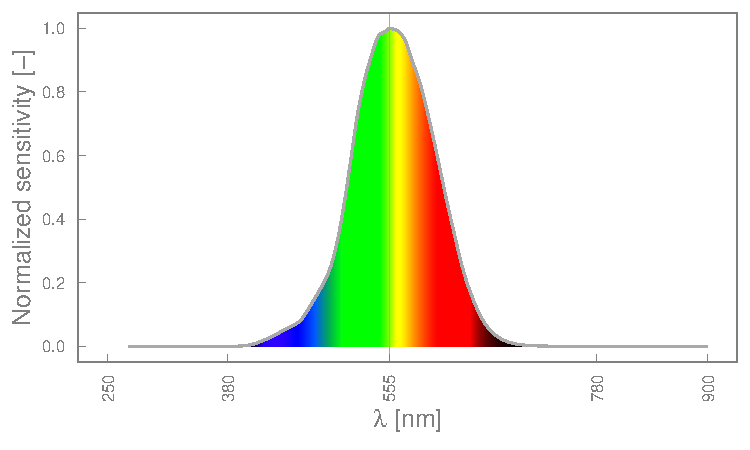
\includegraphics[width=\maxwidth]{figure/Vis_Graph-1} 

}

\DIFdelbeginFL %DIFDELCMD < \caption{%%%
\DIFdelendFL \DIFaddbeginFL \caption[Normalized sensitivity and color perception of the human eye to EM radiation~\cite{schubert2006}, according to the photopic luminous weighting function~($V_\lambda$)]{\DIFaddendFL Normalized sensitivity and color perception of the human eye to EM radiation~\cite{schubert2006}, \mbox{according to} the photopic luminous weighting function~($V_\lambda$). }\label{fig:Vis_Graph}
\end{figure}


\end{knitrout}

The second aspect is to note that 
modern lighting is provided via an energy conversion chain:
primary energy \DIFaddbegin \ins{carriers} \DIFaddend (e.g., coal) \DIFdelbegin \DIFdelend \DIFaddbegin {are} \DIFaddend converted to
final energy (electricity, measured in watts, W) and lastly to
useful energy (visible light, measured in lumens, lm).
\DIFdelbegin \DIFdelend \DIFaddbegin \ins{The field of exergy analysis has long analyzed individual machines
and power plants in the energy conversion chain 
for their exergetic efficiency and performance, e.g.,
co-generation power plants~\cite{Bejan:1996},
nuclear power plants~\cite{Durmayaz:2001}, 
refrigerators~\cite{joybari2013exergy},
heat pumps~\cite{bobbo2019energetic}, and 
energy storage systems~\cite{zwierzchowski2020energy}.
In contrast,} the  field of societal exergy analysis evaluates entire energy conversion chains
at regional, national, or world levels in exergy terms and
considers light (and many other useful energy products)
to be enablers of economic growth.
(Energy quantifies the potential to change temperature,
whereas exergy quantifies the potential to do work).
 See \citet{Nakicenovic1996} for an early example and
\ins{\citet{Guevara:2016a},}
\mbox{%DIFAUXCMD
\citet{Heun:2019aa}, and \citet{Ver-Beek:2020aa}} for later examples
 of societal exergy analysis%DIFDELCMD < \ins{Thus, societal exergy analysis 
%DIFDELCMD < relies upon results from the energy and exergy analysis of 
%DIFDELCMD < lamps and lighting to assess the ways in which useful energy products 
%DIFDELCMD < enable economic growth.}
%DIFDELCMD < %%%
.
Thus, societal exergy analysis 
relies upon results from the energy and exergy analysis of 
lamps and lighting to assess the ways in which useful energy products 
enable economic growth.


Lighting contributes a non-negligible proportion of total useful exergy
supplied to modern economies, so
an essential metric for societal exergy analysis
is the efficiency with which
electricity (final stage) is converted to light (useful stage) by lamps.
Therefore , the efficiency of energy and exergy conversion of electricity
into light by electric lamps~($\eta_E$ and $\eta_X$, respectively)
is the focus of this article.
Note that both energy services (e.g., illumination\DIFdelbegin %DIFDELCMD < \ins{, the stage of the energy conversion chain
%DIFDELCMD < termed ``application efficacy' in photometry \cite{rea2001application}}%%%
, the stage of the energy conversion chain
termed ``application efficacy'' in photometry 
\cite{rea2001application}) 
and satisfaction of human needs
(e.g., comfort, safety, etc.) are downstream of the useful stage 
and thus \DIFdelbegin %DIFDELCMD < \rev{outside of}{beyond the} %%%
%DIFDELCMD < \ins{of this paper}%%%
{beyond the scope of this paper}.


%++++++++++++++++++++++++++++++
\subsection{The Conventional Method and the Thorny Issue of Luminous Efficacy}
\label{sec:conventional_method}
%++++++++++++++++++++++++++++++

The valuable \enoex{} conversion efficiency ($\eta_v$)
is defined in simple terms as
\begin{equation} \label{eq:eta_basic_eqn}
 \eta_v = \frac{\text{valuable output}}{\text{input}} \; .
\end{equation}

When the numerator and denominator are quantified in energy terms,
an energy efficiency is obtained~($\eta_{E,v}$).
When the numerator and denominator are quantified in exergy terms,
an exergetic efficiency is obtained~($\eta_{X,v}$).

But light (the valuable output) is rarely quantified in energy terms
and almost never in exergy terms.
Instead, light is quantified in lumens~(lm).
Indeed, a common interpretation of \mbox{Equation~(\ref{eq:eta_basic_eqn})} uses
light (in lm) as the valuable output in the numerator and 
electricity (in W) as the input in the denominator
to obtain luminous efficacy ($K$, in lm/W).
In fact, most lamps are rated and advertised by their lumen output and their luminous efficacy~($K$).
Figure~\ref{fig:LuminousEfficacy_Graph} shows the evolution over time 
of luminous efficacy for four lamp technologies.
\DIFaddbegin \ins{(Data for Figure~\ref{fig:LuminousEfficacy_Graph} were obtained from three sources: 
the Museum of Electric Lamp Technology (LampTech)~\cite{hooker_2020}, 
the ENERGYSTAR database of certified lamps~\cite{energystar_2020}, and 
the Lighting Market Characterization Reports commissioned by the 
US Department of Energy (DOE)~\cite{DOE2002, DOE2012, DOE2017}).}
\DIFaddend Practitioners who use luminous efficacy 
as a lamp efficiency metric include \citet{Nordhaus1996} and
Tsao and Waide, 
who state 
``[l]uminous efficacy represents the efficiency 
with which energy is used to produce visible light'' \citep{Tsao2010appetitelight} (p.~265).





\begin{knitrout}
\definecolor{shadecolor}{rgb}{0.969, 0.969, 0.969}\color{fgcolor}\begin{figure}[H]

{\centering 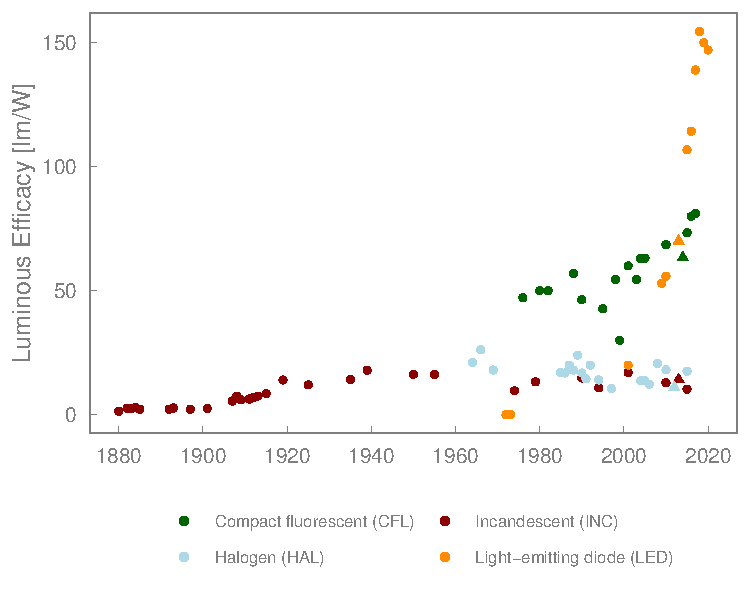
\includegraphics[width=0.65\textwidth]{figure/LuminousEfficacy_Graph-1} 

}

\caption[The luminous efficacy of selected lamp technologies from 1880 to 2020]{The luminous efficacy of selected lamp technologies from 1880 to 2020. Triangles indicate lamps used as examples in this paper.}
\label{fig:LuminousEfficacy_Graph}
\end{figure}


\end{knitrout}

Sousa~{et~al.} %DIF <  \citeauthor{Sousa2017} 
note that 
societal exergy analysis is hampered when 
``the useful output cannot or is not
typically measured in energy units''~\cite{Sousa2017}  (p.~17),
as is the case with lighting.
Indeed, \mbox{societal exergy} practitioners 
need the valuable energy and exergetic efficiencies 
of lamps~($\eta_{E,L,v}$ and $\eta_{X,L,v}$), 
\mbox{but lighting} efficiencies are given in 
terms of luminous efficacy~($K$).
Thus, the widespread use of luminous efficacy~($K$) as a measure of lamp efficiency 
provides a burden to societal exergy analysis.

Conventionally, societal exergy practitioners solve this problem by estimating
the valuable~($v$) exergetic~($X$) efficiency~($\eta$) of lighting~($L$) by the ratio of
the minimum energy required to produce a given output and
the actual energy required to produce the same given output, 
as recommended by \citet{Sousa2017}
for sound, information, and lighting.
(See Section~\ref{sec:previous_approach} for additional detail).
\mbox{The conventional} method is typically implemented 
for lighting via luminous efficacy with
\begin{equation} \label{eq:eta_eqn}
  \eta_{X,L,v} \approx \frac{K}{K_{max}} \; ,
\end{equation}
%
where $K$ is the actual lamp luminous efficacy and 
$K_{max}$ is the theoretical maximum luminous efficacy.

However, Equation~(\ref{eq:eta_eqn}) exposes 
a source of confusion, 
namely what value should be used for $K_{max}$?
Within the societal exergy analysis literature and beyond, 
three common values are adopted: 
\mbox{220~lm/W \cite{Summers1971, Ayres2003, USDepartmentofEnergyDoE2011}},
400 lm/W \cite{Summers1971, Ayres2005, Tsao2010solidstate, Guevara2016}, and
683 lm/W \cite{Kondo2009, Serrenho2014}.
To our knowledge, 
the earliest reference for 220~lm/W and 400~lm/W is 
\citet{Summers1971} (p.~151),
who stated ``[t]he efficiencies \ldots{} assume that the maximum attainable efficiency
for an acceptable white light is about
400 lumens per watt rather than the theoretical value 
of 220 lumens per watt 
for a perfectly `flat' white light''.
\mbox{The value} of 683~lm/W is  %DIFDELCMD < \rev{the maximum efficacy}{derived from the definition of the lumen. 
%DIFDELCMD < It represents the luminous efficacy of a lamp 
%DIFDELCMD < emitting light at 555~nm, the peak of the photopic luminous weighting function, 
%DIFDELCMD < with electricity converted EM radiation at 100\% efficiency.}
%DIFDELCMD < %%%
derived from the definition of the lumen. 
It represents the luminous efficacy of a lamp 
emitting light at 555~nm, the peak of the photopic luminous weighting function, 
with electricity converted EM radiation at 100\% efficiency.


Paoli and Cullen
estimated the practical upper limit for the luminous efficacy of an LED lamp to be 284--350~lm/W,
when considering all  %DIFDELCMD < \rev{stages}{sources} %%%
sources  of energy loss
\DIFdelbegin %DIFDELCMD < \ins{(driver efficiency, wall plug efficiency, optical efficiency, and spectral efficiency)}%%%
(driver efficiency, wall plug efficiency, optical efficiency, and spectral efficiency)~\citep{Paoli2020}.
The development of LED technology is following Haitz's law, 
which predicts that ``[e]very decade, for a given wavelength of light, 
the cost per lumen falls by a factor of 10 
and the amount of light generated per LED package increases 
by a factor of 20''~\citep{haitz1999case, graydon2007haitz}.
Figure~\ref{fig:LuminousEfficacy_Graph} shows that 
 %DIFDELCMD < \ins{LED technology is nearing} %%%
LED technology is nearing  the 
lower efficacies from Summers (220 lm/W) and
Paoli and Cullen (284 lm/W).
\DIFdelbegin %DIFDELCMD < \del{are within reach,
%DIFDELCMD < due to the rapid improvement of LED technology.}
%DIFDELCMD < %%%
\DIFdelend 

Clearly, there are many options for $K_{max}$, and
its value has a large effect on the valuable exergetic efficiency of lighting
in the conventional method (Equation~(\ref{eq:eta_eqn})).
So getting it right is important.


%++++++++++++++++++++++++++++++
\subsection{Need, Aim, Contributions, and Structure}
\label{sec:aim_contribution_structure}
%++++++++++++++++++++++++++++++

Although the confusion around maximum luminous efficacy~($K_{max}$)
is sufficient motivation to dig deeper to fully understand and define
the exergy of light and the exergetic efficiency of lamps, 
\mbox{further issues} and confusions await. 
(See Section~\ref{sec:discussion}).
Thus, there is ample \emph{need} for clarity and rigor 
about the thermodynamics of artificial lighting.

The need leads to the \emph{aim} of this article: 
to bring clarity to 
%
\begin{enumerate*}[label={(\alph*)}]

  \item the energy and exergy of light and        

  \item the valuable energy and exergetic efficiency of lamps

\end{enumerate*}
%
for societal exergy analysis.

The novel \emph{contributions} of this article include:
%
\begin{enumerate*}[label={(\alph*)}]

  \item clear and rigorous definitions of the energy and exergy of light, 
        applicable to the field of
        societal exergy analysis~(Section~\ref{sec:phi_light}),

  \item presentation of a framework for understanding 
        the exergetic efficiency of lamps
        (the exact method, Section~\ref{sec:light_efficiency}),

  \item application of the exact method to re-interpret the conventional method,
        \mbox{exposing its} shortcomings~(Section~\ref{sec:previous_approach}),

  \item recommendations for societal exergy analysis going forward (Section~\ref{sec:recommendations}), and 

  \item development of an approximate method for cases when an approximation to the exact method is needed
        (Section~\ref{sec:approximate_method}).

\end{enumerate*}

The \emph{structure} of this article is as follows:
In Section~\ref{sec:methods}, we 
%
\begin{enumerate*}[label={(\alph*)}]

  \item set out the energy and exergy fundamentals of light and lighting efficiency and

  \item define luminous weighting functions and spectral power distributions for example lamps.

\end{enumerate*}
%
In Section~\ref{sec:results}, we show results for luminous weighting functions and example lamps before
presenting a discussion in Section~\ref{sec:discussion}.
Section~\ref{sec:conclusions} summarizes and {suggest future work}\DIFaddend .


%%%%%%%%%%%%%%%%%%%%%%%%%%%%%%%%%%%%%%%%%%%%%%%%%%%%%%%%%%%%%%
\section{Methods}
\label{sec:methods}
%%%%%%%%%%%%%%%%%%%%%%%%%%%%%%%%%%%%%%%%%%%%%%%%%%%%%%%%%%%%%% 

%DIF <  Materials and Methods should be described with sufficient details 
%DIF <  to allow others to replicate and build on published results. 
%DIF <  Please note that publication of your manuscript implicates 
%DIF <  that you must make all materials, data, computer code, and protocols
%DIF <  associated with the publication available to readers. 
%DIF <  Please disclose at the submission stage any restrictions 
%DIF <  on the availability of materials or information. 
%DIF <  New methods and protocols should be described 
%DIF <  in detail while well-established methods 
%DIF <  can be briefly described and appropriately cited.
%DIF <  
%DIF <  Research manuscripts reporting large datasets that are deposited
%DIF <  in a publicly available database should specify 
%DIF <  where the data have been deposited and provide the relevant accession numbers. 
%DIF <  If the accession numbers have not yet been obtained at the time of submission, 
%DIF <  please state that they will be provided during review. 
%DIF <  They must be provided prior to publication.
%DIF <  
%DIF <  Interventionary studies involving animals or humans, and other studies
%DIF <  require ethical approval must list the authority 
%DIF <  that provided approval and the corresponding ethical approval code. 
\DIFdelbegin %DIFDELCMD < 
\vspace{-6pt}

%DIFDELCMD < %%%
\DIFdelend %++++++++++++++++++++++++++++++
\subsection{Exergy Theory}
\label{sec:framework}
%++++++++++++++++++++++++++++++

Energy and exergy are two ways to quantify the physical property that,
when transferred to an object,
changes its temperature or performs work on it.
(In this section, we can't call the ``physical property'' energy, exergy, work, or heat,
because these concepts must remain apart,
so we use the generic term ``physical property'').
We discuss energy and exergy quantifications of the physical property in the sections below, 
beginning with heat and work, 
the concepts for which \enaex{} originated.
Thereafter, we develop a framework for the \enaex{} of light
that parallels the \enaex{} of heat and work.


%------------------------------
\subsubsection{Energy and Exergy ($\dot{E}$ and $\dot{X}$) of Heat and Work} 
\label{sec:energy_and_exergy_of_heat_and_work}
%------------------------------

Energy quantifies the physical property by its heat content.
Thus, heat (the ability to influence temperature) is pure energy.
Thanks to Thompson's cannon experiment~\cite{Thompson:1798aa}, 
we know that work can be converted into heat without loss.

Figure~\ref{fig:heat_engine} shows a heat engine that converts 
heat at \Circled{1} to 
work at \Circled{3}
with a waste heat byproduct at \Circled{2}. 
All streams can be counted as energy ($\dot{E}$), such that 
\begin{align}
  \dot{E}_1 &= \dot{Q}_1, \\
  \dot{E}_2 &= \dot{Q}_2, \; \text{and} \\
  \dot{E}_3 &= \dot{W}_3 \; .
\end{align}
%
%MDPI: Please check if it can be deleted.
% Do not delete!
Note that the overdot notation, as in $\dot{E}$, $\dot{Q}$, and $\dot{W}$,
indicates a steady state rate of energy or \mbox{exergy flow.}

\begin{figure}[H]
\centering
\begin{tikzpicture}
  % Set up the nodes of the main path
  % Machine node
  \node(machine)[draw, rounded corners, fill=yellow!25!white, 
                 minimum width = 3 cm, minimum height = 2 cm] at (0cm, 0cm) {\strut Heat engine};
  % Number nodes
  \node[left=3cm of machine] (1)[circle, fill=red!25!white] {\strut 1};
  \node[above right = -0.7cm and 3cm of machine] (2)[circle, fill=red!25!white] {\strut 2};
  \node[below right = -0.7cm and 3cm of machine] (3)[circle, fill=red!25!white] {\strut 3};
  % Arrows
  \draw[arrows=-triangle 45] (1) -- node [above] {$\dot{Q}_1, T_1$} (machine);
  \draw[arrows=-triangle 45] (2 -| machine.east) -- node [above] {$\dot{Q}_2$, $T_2$} (2.west);
  \draw[arrows=-triangle 45] (3 -| machine.east) -- node [below] {$\dot{W}_3$} (3.west);
\end{tikzpicture}
\caption{A heat engine that uses heat at \Circled{1} to produce heat at \Circled{2} and work at \Circled{3}.}
\label{fig:heat_engine}
\end{figure}

Energy efficiency is defined as $\eta_E \equiv \frac{\text{energy out}}{\text{energy in}}$.
For the example of Figure~\ref{fig:heat_engine}, 
\begin{equation} \label{eq:energy_efficiency}
  \eta_E = \frac{\dot{E}_2 + \dot{E}_3}{\dot{E}_1} = \frac{\dot{Q}_2 + \dot{W}_3}{\dot{Q}_1} = 1 \; ,
\end{equation}
%
because the first law of thermodynamics requires
that energy is conserved ($\dot{Q}_1 = \dot{Q}_2 + \dot{W}_3$).

That said, typically only one of the products in Figure~\ref{fig:heat_engine} 
is deemed valuable: the work produced by the heat engine ($\dot{W}_3$).
Thus, the \emph{valuable} energy efficiency ($\eta_{E,v}$) is 
\begin{equation} \label{eq:valuable_energy_efficiency}
  \eta_{E,v} = \frac{\dot{E}_3}{\dot{E}_1} = \frac{\dot{W}_3}{\dot{Q}_1} < 1 \; .
\end{equation}

Heat (the ability to influence temperature) is 
only one possible outcome of transferring the physical property
from one object to another.
Heat is certainly valuable to humans, but so is another property: 
work, the ability to exert a force on another object.
Exergy quantifies the physical property by its work potential
and provides the answer to the question
``what is the maximum work we could obtain from a stream of \DIFdelbegin %DIFDELCMD < \rev{this}{the} %%%
the  physical property''?
Thus, work is pure exergy.

The Kelvin-Planck statement of the second law of thermodynamics 
states that heat cannot be converted to work without loss. 
To find the maximum possible work that can be created from heat 
(and, therefore, the exergy of heat), 
we require the Carnot heat engine, which operates
at the maximum possible valuable energy efficiency~($\eta_C$).
\begin{equation} \label{eq:eta_C}
  \eta_C = 1 - \frac{T_0}{T_{sys}}
\end{equation}
%
$T_0$ is the ambient temperature, and $T_{sys}$ is a heat temperature 
($T_1$ or $T_2$ in Figure~\ref{fig:heat_engine}).
The exergy of each stream in Figure~\ref{fig:heat_engine} is then
\begin{align}
  \dot{X}_1 &= \phi_1 \dot{Q}_1 = \left(1 - \frac{T_0}{T_1} \right) \dot{Q}_1, \\
  \dot{X}_2 &= \phi_2 \dot{Q}_2 = \left(1 - \frac{T_0}{T_2} \right) \dot{Q}_2, \text{ and} \\
  \dot{X}_3 &= \cancelto{1}{\phi_3} \dot{W}_3 = \dot{W}_3 \; .
\end{align}

In this context, the Carnot efficiency~($\eta_C$) becomes the exergy-to-energy ratio
for heat streams ($\phi_Q = \eta_C$).
The exergy-to-energy ratio for work is $\phi_3 = \phi_W = 1$, 
because work is pure exergy.
\mbox{(The exergy-to-energy ratio}, $\phi$,
is exergy divided by energy at a statepoint.
E.g., $\phi_1 = \dot{X}_1 / \dot{E}_1$).

The exergetic efficiency of an energy conversion device 
is defined as $\eta_X \equiv \frac{\text{exergy out}}{\text{exergy in}}$.
For the heat engine in Figure~\ref{fig:heat_engine}, 
\begin{equation} \label{eq:exergy_efficiency}
  \eta_X = \frac{\dot{X}_2 + \dot{X}_3}{\dot{X}_1} = \frac{\dot{Q}_2 \left( 1 - \frac{T_0}{T_2} \right)  + \dot{W}_3}{\dot{Q}_1 \left( 1 - \frac{T_0}{T_1} \right) } < 1 \; ,
\end{equation}
%
\DIFdelbegin %DIFDELCMD < \del{because the second law of thermodynamics 
%DIFDELCMD < states that exergy is always destroyed ($\dot{X}_1 > \dot{X}_2 + \dot{X}_3$ or 
%DIFDELCMD < $\dot{X}_D = \dot{X}_1 - (\dot{X}_2 + \dot{X}_3)$).}
%DIFDELCMD < \ins{because all real processes are internally irreversible, such that 
%DIFDELCMD < $\dot{X}_1 > \dot{X}_2 + \dot{X}_3$ or 
%DIFDELCMD < $\dot{X}_D = \dot{X}_1 - (\dot{X}_2 + \dot{X}_3)$.}
%DIFDELCMD < %%%
because all real processes are internally irreversible, such that 
$\dot{X}_1 > \dot{X}_2 + \dot{X}_3$ or 
$\dot{X}_D = \dot{X}_1 - (\dot{X}_2 + \dot{X}_3)$.

Assuming, again, that work is the valuable output gives
\begin{equation} \label{eq:valuable_exergy_efficiency}
  \eta_{X,v} = \frac{\dot{W}_3}{\dot{Q}_1 \left( 1 - \frac{T_0}{T_1} \right) } < \eta_X < 1\; .
\end{equation}

Note that both $\eta_{E,v}$ and $\eta_{X,v}$ 
are independent of human presence.
The work created by the heat engine~($\dot{W}_3$) could be 
a spinning driveshaft on an automobile carrying four passengers down the freeway or
the same spinning driveshaft on a dynamometer in an unoccupied laboratory.
Both
%
\begin{enumerate*}[label={(\alph*)}]

  \item the \enaex{} of the work and heat at \Circled{2} and \Circled{3} and

  \item the \enaex{} efficiencies of the heat engine ($\eta_{E,v}$ and $\eta_{X,v}$)

\end{enumerate*}
%
would be the same, regardless.
In other words, both 
%
\begin{enumerate*}[label={(\alph*)}]

  \item the \enaex{} of work and heat and

  \item the efficiencies of the heat engine

\end{enumerate*}
%
are independent of human presence and the energy service provided by the heat engine.

We now turn 
from the production of work by a heat engine
to the production of light by a lamp.


%------------------------------
\subsubsection{Energy and Exergy of EM Radiation ($\dot{E}_{EM}$ and $\dot{X}_{EM}$)} 
\label{sec:energy_and_exergy_of_EM_rad}
%------------------------------

Figure~\ref{fig:lamp} replaces the heat engine with a lamp 
that produces broad-spectrum EM radiation~($\dot{E}_{EM,3}$)
instead of work~($\dot{W}_3$).
Electricity powers the lamp at \Circled{1}, and,
like Figure~\ref{fig:heat_engine},
waste heat (conduction and convection only) is produced at \Circled{2}.

\begin{figure}[H]
\centering
\begin{tikzpicture}
  % Set up the nodes of the main path
  % Machine node
  \node(machine)[draw, rounded corners, fill=yellow!25!white, 
                 minimum width = 3 cm, minimum height = 2 cm] at (0cm, 0cm) {\strut Lamp};
  % Number nodes
  \node[left=2cm of machine] (1)[circle, fill=red!25!white] {\strut 1};
  \node[above right = -0.7cm and 2cm of machine] (2)[circle, fill=red!25!white] {\strut 2};
  \node[below right = -0.7cm and 2cm of machine] (3)[circle, fill=red!25!white] {\strut 3};

  \node(wf)[draw, rounded corners, fill=yellow!25!white, 
            minimum width = 3 cm, minimum height = 2 cm,
            align = center, right = 1 cm of 3] {\strut Weighting\\function ($f_{\lambda}$)};

  \node[above right = -0.7 cm and 2 cm of wf] (4)[circle, fill=red!25!white] {\strut 4};
  \node[below right = -0.7 cm and 2 cm of wf] (5)[circle, fill=red!25!white] {\strut 5};

  % Arrows
  \draw[arrows=-triangle 45] (1) -- node [above] {$\dot{W}_{elect,1}$} (machine);
  \draw[arrows=-triangle 45] (2 -| machine.east) -- node [above] {$\dot{Q}_2$, $T_2$ } (2.west);
  \draw[arrows=-triangle 45] (3 -| machine.east) -- node [below] {$\dot{E}_{EM,3}$} (3.west);
  \draw[arrows=-triangle 45] (wf -| 3.east) -- node [below] {} (wf.west);
  \draw[arrows=-triangle 45] (4 -| wf.east) -- node [above] {$\dot{E}_{N,4}$} (4.west);
  \draw[arrows=-triangle 45] (5 -| wf.east) -- node [below] {$\dot{E}_{L,5}$} (5.west);

\end{tikzpicture}
\caption{A lamp that uses electricity at \Circled{1} to produce
         heat at \Circled{2}, broad-spectrum EM radiation at \Circled{3}, 
         non-light EM radiation at \Circled{4}, and light at \Circled{5}.}
\label{fig:lamp}
\end{figure}

Both electricity and EM radiation can be converted to heat without loss, so they are pure \mbox{energy.
Thus,}
\begin{align}
  \dot{E}_1 &= \dot{W}_{elect,1}, \\
  \dot{E}_2 &= \dot{Q}_2, \; \text{and} \\
  \dot{E}_3 &= \dot{E}_{EM,3} \; ,
\end{align}
%
where $\dot{E}_{EM,3}$ is the radiant power of broad-spectrum EM radiation
emitted by the lamp in units of energy per unit time~(W).
(Confusingly, radiant power is sometimes called ``radiant flux'' in the literature,
despite the fact that radiant power is in units of W,
whereas flux would be in units of $\text{W} \! /\text{m}^2$.
When exergy is not involved, the photometry literature often denotes
radiant power by $\Phi$, not $\dot{E}$.
Here, we need to differentiate between 
the energy rate of broad spectrum EM radiation~($\dot{E}_{EM}$) and
the exergy rate of broad spectrum EM radiation~($\dot{X}_{EM}$),
so we reserve $\Phi$ for lumen output of a lamp. 
\mbox{See Section~\ref{sec:weighting_functions}}).

The lamp's energy efficiency~($\eta_{E,EM}$) is 
\begin{equation}  
  \eta_{E,EM} = \frac{\dot{E}_2 + \dot{E}_3}{\dot{E}_1} = \frac{\dot{Q}_2 + \dot{E}_{EM,3}}{\dot{W}_{elect,1}} = 1 \; .
\end{equation}

\textls[-20]{The valuable energy efficiency of the lamp
in Figure~\ref{fig:lamp}~($\eta_{E,EM,v}$, also called the wall plug efficiency)
is}
\begin{equation} \label{eq:eta_E_v}
  \eta_{E,EM,v} = \frac{\dot{E}_3}{\dot{E}_1} = \frac{\dot{E}_{EM,3}}{\dot{W}_{elect,1}} < 1 \; ,
\end{equation}
%
assuming that broad-spectrum EM radiation at \Circled{3} is the valuable output from the lamp.

Because electricity can be converted to work without loss in a frictionless motor,
electricity is considered pure exergy, i.e., $\phi_{elect} = 1$.
Thus, the exergy of the first three streams in Figure~\ref{fig:lamp} is given by 
\begin{align}
  \dot{X}_1 &= \cancelto{1}{\phi_{elect}} \dot{W}_{elect,1} = \dot{W}_{elect,1}, \\
  \dot{X}_2 &= \left( 1 - \frac{T_0}{T_2} \right) \dot{Q}_2, \; \text{and} \\
  \dot{X}_3 &= \phi_{\EM} \dot{E}_{EM,3} \; ,
\end{align}
%
where $\phi_{EM}$ is the exergy-to-energy ratio for broad-spectrum EM radiation. 
(See Section~\ref{sec:phi_light} \mbox{for details}).

In general, the radiant power of a lamp is a spectral quantity,
meaning that it varies with wavelength.
Spectral radiant power~($\dot{E}_{EM,\lambda}$)
is the EM emissive power available between any two wavelengths
and is related to radiant power~($\dot{E}_{EM}$) by
\begin{equation} \label{eq:emissive_power}
  \dot{E}_{EM} = \int \dot{E}_{EM,\lambda} \mathrm{d}\lambda \; .
\end{equation}
%
(See~\citet{benenson2006handbook}.) Visually, $\dot{E}_{EM}$ is the area under the $\dot{E}_{EM,\lambda}$ vs.\ $\lambda$ curve.%mdpi:Please fill in the brackets

The exergetic efficiency of EM radiation emitted by the lamp in Figure~\ref{fig:lamp} is given by
\begin{equation}
  \eta_{X,EM} = \frac{\dot{X}_2 + \dot{X}_3}{\dot{X}_1} 
          = \frac{\left( 1 - \frac{T_0}{T_2} \right) \dot{Q}_2 + \phi_{EM} \dot{E}_{EM,3} }{\dot{W}_{elect,1}} < 1 \; ,
\end{equation}

In general, $\phi_{EM}$ is also a spectral quantity.
(See Section~\ref{sec:phi_light}).
The valuable exergetic efficiency of the EM radiation emitted by the lamp in Figure~\ref{fig:lamp} is given by
\begin{equation} \label{eq:eta_X_v}
  \eta_{X,EM,v} = \frac{\dot{X}_3}{\dot{X}_1} 
              = \frac{\phi_{EM} \dot{E}_{EM,3} }{\dot{W}_{elect,1}} < \eta_{X,EM} < 1 \; .
\end{equation}

Note that the efficiencies are independent of human presence;
$\eta_{X,EM}$ and $\eta_{X,EM,v}$ would be the same, 
whether the lamp is illuminating
an unoccupied room or a crowded bar, or
whether the illumination stimulates the rods and cones of a human eye or
excites band gap electrons in an amorphous silicon solar cell.


%------------------------------
\subsubsection{Energy and Exergy of Light ($\dot{E}_{L}$ and $\dot{X}_{L}$)} 
\label{sec:human_perception_of_EM_radiation}
%------------------------------

We noted above that both
%
\begin{enumerate*}[label={(\alph*)}]

  \item \enaex{} of broad-spectrum EM radiation and

  \item EM energy and exergetic efficiency of lamps

\end{enumerate*}
%
are independent of human presence.
But what about \mbox{human \emph{perception}?}

Human beings perceive conductive and convective heat by temperature and EM radiation by wavelength.
Human skin can perceive the thermal radiation portion of the broader electromagnetic spectrum,
approximately 100 nm < $\lambda$ < 10,000 nm, and 
human skin is differentially responsive to EM wavelength~\citep{Anderson:1981aa}.  
Indeed, thermoreceptors in the dermis of skin are important sensors
for regulation of body temperature~\cite{Jones:2016aa} (p.~258). Similarly, human eyes perceive only a (narrower) portion of the EM radiation spectrum
(approximately \humaneyesensitivity).
To quantify the energy (and exergy) of light, 
we must move from the \enaex{} of broad-spectrum EM radiation~($\dot{E}_{EM}$ and $\dot{X}_{EM}$)
to the \enaex{} of light~($\dot{E}_{L}$ and $\dot{X}_{L}$). 
But how?

Knowing that visual perception of light is a function of wavelength
leads to modifying Equation~(\ref{eq:emissive_power})
to include a spectral luminous weighting function~($f_\lambda$) such that
\begin{equation} \label{eq:weighted_emissive_power}
  \dot{E}_L = \int \dot{E}_{L,\lambda} \mathrm{d}\lambda = \int f_\lambda \dot{E}_{EM,\lambda} \mathrm{d}\lambda \; ,
\end{equation}
%
with $0 \le f_\lambda \le 1$
and $\dot{E}_{L,\lambda} = f_\lambda \dot{E}_{EM,\lambda}$.

In Equation~(\ref{eq:weighted_emissive_power}), 
the spectral luminous weighting function~($f_\lambda$) converts 
broad-spectrum EM radiation~($\dot{E}_{EM}$ and $\dot{X}_{EM}$)
to light~($\dot{E}_{L}$ and $\dot{X}_{L}$), 
the valuable part of EM radiation for illumination.
\mbox{In the} context of Figure~\ref{fig:lamp}, 
\begin{equation} \label{eq:L_dot_5}
  \dot{E}_{L,5} = \int f_\lambda \dot{E}_{EM,\lambda,3} \, \mathrm{d}\lambda \; .
\end{equation}

In Figure~\ref{fig:lamp}, any EM radiation at statepoint 3 
\emph{not} converted to light
is quantified as non-light EM radiation at statepoint 4~($\dot{E}_{N,4}$).
Specifically,
\begin{equation} \label{eq:N_dot_5}
  \dot{E}_{N,4} = \int (1 - f_\lambda) \dot{E}_{EM,\lambda,3} \, \mathrm{d}\lambda \; .
\end{equation}


%------------------------------
\subsubsection{The Exergy-To-Energy Ratio of EM Radiation ($\phi_{\EM}$)}
\label{sec:phi_light}
%------------------------------

Recent advances in the thermodynamics of radiation community
enable converting the energy of EM radiation~($\dot{E}_{EM}$)
into the exergy of EM radiation~($\dot{X}_{EM}$)~\cite{Shan2019}.
The exergy-to-energy ratio of EM radiation
($\phi_{\EM}$, called the ``radiative exergy-energy coefficient'' in that community)
is most commonly given by Petela's Equation~\cite{petela1964exergy, Delgado-Bonal:2017aa, Shan2019}:
\vspace{-12pt}
\begin{equation} \label{eq:petelas_equation}
 \phi_{\EM} = 1 - \frac{4}{3}\frac{T_{0}}{T_{1}} + \frac{1}{3} \left(\frac{T_{0}}{T_{1}}\right)^4 \; ,
\end{equation}
%
where $T_1$ is the temperature of a blackbody emitter and 
$T_0$ is the temperature of a blackbody absorber.
Petela's equation has recently been verified via an infinite-staged
Carnot heat engine model \cite{zhou2017exergy}
that is powered by radiative energy transfer.
In the radiative Carnot model, a photon possessing a characteristic frequency 
and photon effective temperature enters a medium that acts as an ideal absorber. 
The photon transfers an infinitesimal quantity of energy to the absorber via thermal radiation.
The energy enters an infinitesimally small Carnot heat engine and performs work. 
The absorber then emits another photon at lower energy and frequency,
and therefore lower photon effective temperature. 
This process repeats until the frequency of the photon is zero
and the photon effective temperature~($T_\lambda$)
equals the reference temperature ($T_0$)~\cite{Shan2019}.

However, Petela's equation assumes a blackbody emitter~(at $T_1$) and
a blackbody absorber~(at $T_0$).
To determine $\phi_{\EM}$ for an emitter that is a non-blackbody lamp,
the spectral exergy-to-energy ratio ($\phi_{\EM,\lambda}$),
must be calculated.
Recently, 
Delgado-Bonal
% \citeauthor{Delgado-Bonal:2017aa} 
was the first to quantify
the spectral entropy of radiation, which 
reduces to Petela's equation when the full spectrum is considered~\citep{Delgado-Bonal:2017aa}.
Here, \mbox{we use} an effective temperature of light photons~\cite{chen2008} ($T_\lambda$) 
to obtain the link between Petela's equation (Equation~(\ref{eq:petelas_equation}))
and the spectral exergy-to-energy ratio~($\phi_{\EM,\lambda}$).
The product of wavelength and photon effective temperature 
is a constant~($c_3$ in \citet{chen2008}) such that
\begin{equation}
  \lambda T_{\lambda} = c_{3} = 5.33016 \times 10^{-3} \text{ m-K} \; ,
\end{equation}
%
or
\begin{equation} \label{eq:T_lambda}
  T_\lambda = \frac{c_3}{\lambda} = \frac{5.33016 \times 10^{-3} \text{ m-K}}{\lambda} \; .
\end{equation}

We note that the photon effective temperature approach has been criticized by 
Liu,
% \citeauthor{liu2009},
who argued that it is inappropriate
``to endue a single photon with macro-scale thermodynamic parameters
such as exergy and entropy''~\citep{liu2009} (p.~1810).  We acknowledge this critique, 
but we also note that here $T_\lambda$ is ascribed to a stream of photons
traveling from a lamp to an eye.
Thus, for our purposes, $T_\lambda$ can be considered the statistical average effective temperature 
of that stream of photons,
in accordance with~\citet{Shan2019}.

We assume that the mechanism
by which light is converted into electrical nerve signals
in the human eye
is radiative EM energy transfer
from a light source~(1) to an eye~(0).
We assume no losses in radiative transmission
between the lamp and the iris,
i.e., no radiation scattering occurs through air, 
\mbox{an assumption} that holds for short distances typically 
observed in lighting applications (<~10~m).
(\mbox{See \citet{Shan2019}} for a method to estimate transmission losses
over longer distances).
\mbox{We further} assume that the human iris is a blackbody absorber 
(absorbing all wavelengths of radiation perfectly \cite{benenson2006handbook}), 
being a small aperture on a larger cavity.
(In this assumption, we follow  \citet{Rossing2020}  (p.~172)who state
``another good example of [a blackbody absorber] is the human eye;
the pupil looks black because most light entering it is trapped and absorbed'').
Thus, we use Shan and Zhou's~\cite{Shan2019} spectral formulation of Petela's equation,
which replaces the temperature of the emitter ($T_1$) by photon effective temperature~($T_\lambda$):
\begin{equation} \label{eq:phi_EM_lambda_shan_zhou}
 \phi_{\EM,\lambda} = 1 - \frac{4}{3} \left( \frac{T_{0}}{T_{\lambda}} \right)
                        + \frac{1}{3} \left(\frac{T_{0}}{T_{\lambda}}\right)^4 \; .
\end{equation}

Further, Equation~(\ref{eq:T_lambda}) (in the form $T_\lambda = c_3 / \lambda$)
can be substituted into Equation~(\ref{eq:phi_EM_lambda_shan_zhou}),
and $T_0$ can be taken as 310~K, the temperature of the human body.
The result is an equation for $\phi_{L,\lambda}$, the spectral exergy-to-energy ratio of light:

\begin{equation} \label{eq:phi_L_lambda_shan_zhou}
 \phi_{L,\lambda} = 1 
                    - \frac{4}{3} \left( \frac{310 \text{ K}}{c_3} \right) \lambda 
                    + \frac{1}{3} \left( \frac{310 \text{ K}}{c_3} \right)^4 \lambda^4 \; .
\end{equation}

The exergy of light emitted by a non-blackbody lamp~($\dot{X}_L$)
is found by integrating the product of
the spectral radiant power~($\dot{E}_{EM,\lambda}$),
a spectral luminous weighting function~($f_\lambda$), and
the spectral exergy-to-energy ratio~($\phi_{L,\lambda}$)
with respect to wavelength.

\begin{equation} \label{eq:X_dot_L}
  \dot{X}_L = \int \phi_{L,\lambda} \, f_\lambda \, \dot{E}_{EM,\lambda} \mathrm{d}\lambda
\end{equation}

The quotient of $\dot{X}_L$ and $\dot{E}_L$ gives 
the exergy-energy ratio of light~($\phi_{L}$), 
which is specific to each combination of
weighting function and lamp ($f_\lambda \dot{E}_{EM,\lambda}$).

\begin{equation} \label{eq:phi_L}
  \phi_{L} = \frac{\dot{X}_L}{\dot{E}_L} 
           = \frac {\int \phi_{L,\lambda} f_\lambda \dot{E}_{EM,\lambda} \mathrm{d}\lambda}
                       {\int f_\lambda \dot{E}_{EM,\lambda} \mathrm{d}\lambda}
\end{equation}

Table~\ref{tab:EX_summary} summarizes the key equations in 
Sections~\ref{sec:energy_and_exergy_of_heat_and_work}--\ref{sec:phi_light}.

\begin{table}[H]
\centering % Centered table
\caption{Summary of equations for energy and exergy of work, electricity, heat, EM radiation, \mbox{and light.}
         $T_0$ is the environment temperature, $T_1$ is the temperature of heat, 
         and $T_\lambda$ is the photon effective temperature
         (Equation~(\ref{eq:T_lambda})).
         Note that $\dot{X} = \phi \dot{E}$ 
         on a spectral basis, if needed.}
\scalebox{0.9}[0.9]{
\begin{tabular}{cccc}
  \toprule
  \textbf{Quantity} 
      & \boldmath{\textbf{Energy Rate~($\dot{E}$)}}
      & \boldmath{\textbf{Exergy-To-Energy Ratio~($\phi$) }}
      & \boldmath{\textbf{Exergy Rate~($\dot{X}$)}} \\
  \midrule
  Work        
      & $\dot{E}_W = \dot{W}$
      & $\phi_W = 1$
      & $\dot{X}_W = \dot{W}$ \\
  %
  Electricity 
      & $\dot{E}_{elect} = \dot{W}_{elect}$
      & $\phi_{elect} = 1$
      & $\dot{X}_{elect} = \dot{W}_{elect}$ \\
  %
  Heat 
      & $\dot{E}_Q = \dot{Q}$   
      & $\phi_Q = 1 - \frac{T_0}{T_1}$  
      & $ \dot{X}_Q = \left( 1 - \frac{T_0}{T_1} \right) \dot{Q}  $ \\
  %
  EM rad.
      & $\dot{E}_{\EM} = \int \dot{E}_{EM,\lambda} \mathrm{d}\lambda$ 
      & $\phi_{\EM{},\lambda} = \petella{T_0}{T_\lambda}$ 
      & $\dot{X}_{\EM} = \int \phi_{\EM,\lambda} \dot{E}_\lambda \mathrm{d}\lambda$ \\
  % 
  Light
      & $\dot{E}_L = \int f_\lambda \dot{E}_{EM,\lambda} \mathrm{d}\lambda$
      & $\phi_{L,\lambda} = 1 
                            - \frac{4}{3} \left( \frac{310 \text{ K}}{c_3} \right) \lambda 
                            + \frac{1}{3} \left( \frac{310 \text{ K}}{c_3} \right)^4 \lambda^4$ % \phi_{\EM{},\lambda}$ 
      & $\dot{X}_L = \int \phi_{L,\lambda} f_\lambda \dot{E}_{EM,\lambda} \mathrm{d}\lambda$ \\
  \bottomrule
\end{tabular}}
\label{tab:EX_summary}
\end{table}


%------------------------------
\subsubsection{Lighting Efficiency of a Lamp} 
\label{sec:light_efficiency}
%------------------------------

If the valuable product of a lamp is considered to be its light~($\dot{E}_L$ or $\dot{X}_L$)
as opposed to its broad-spectrum EM radiation~($\dot{E}_{EM}$ or $\dot{X}_{EM}$),
Equations~(\ref{eq:eta_E_v}) and~(\ref{eq:eta_X_v}) require modification.
In the context of Figure~\ref{fig:lamp}, the valuable energy efficiency of a lamp becomes
\begin{equation} \label{eq:eta_E_v_light}
  \eta_{E,L,v} = \frac{\dot{E}_5}{\dot{E}_{elect,1}} 
               = \frac{\int f_\lambda \dot{E}_{EM,\lambda,3} \, \mathrm{d}\lambda}{\dot{W}_{elect,1}} \; ,
\end{equation}
%
and the valuable exergetic efficiency of a lamp becomes
\begin{equation} \label{eq:eta_X_v_light}
  \eta_{X,L,v} = \frac{\dot{X}_5}{\dot{X}_{elect,1}} 
               = \frac{\int \phi_{L,\lambda} f_\lambda \dot{E}_{EM,\lambda,3} \, \mathrm{d}\lambda}{\dot{W}_{elect,1}} \; .
\end{equation}


%++++++++++++++++++++++++++++++
\subsection{Examples and Data}
\label{sec:examples_and_data}
%++++++++++++++++++++++++++++++
\vspace{-6pt}

%------------------------------
\subsubsection{Luminous Weighting Functions}
\label{sec:weighting_functions}
%------------------------------

Spectral luminous weighting functions ($f_\lambda$) convert 
radiant power ($\dot{E}_{EM}$ and $\dot{X}_{EM}$)
to light ($\dot{E}_L$ and $\dot{X}_L$).
(See Section~\ref{sec:human_perception_of_EM_radiation}).
We use four spectral luminous weighting functions relevant to illumination
to enable example calculations.
(See Section~\ref{sec:results}).

The first luminous weighting function option is degenerate: 
the practitioner could decide to ignore the nuances of human visual perception altogether,
implicitly assuming that all EM radiation emitted from a lamp counts as light, 
whether or not it is within the visible portion of the EM spectrum.
For the first option, the degenerate (unweighted, uw) 
luminous weighting function ($f_{\lambda,uw}$) is
\begin{equation} \label{eq:f1}
  f_{\lambda,uw} = 1 \; .
\end{equation}

Second, the practitioner could 
deem a lamp's EM radiation to be useful if and only if it \emph{could}
stimulate photoreceptive cells in the human eye,
regardless of the spectral sensitivity of those cells.
In the second option, the practitioner excludes wavelengths outside the range of perception by the human eye
when determining the \enoex{} of light.
For the second option (visible, vis),
\begin{equation} \label{eq:f2}
f_{\lambda,vis} =
  \begin{cases}
    0 \; , & \text{for } \lambda < 380 \text{ nm} \\
    1 \; , & \text{for } 380 \text{ nm} \le \lambda \le 780 \text{ nm} \\
    0 \; , & \text{for } 780 \text{ nm} < \lambda \\
  \end{cases} \; .
\end{equation}

But the human eye is spectrally sensitive to EM radiation, 
with peak sensitivity at 555~nm 
\DIFdelbegin %DIFDELCMD < \del{(green)}
%DIFDELCMD < %%%
\DIFdelend and lesser sensitivities at both 
longer (redder, $\lambda > \; \sim{}620 \text{ nm}$) and
shorter (bluer, $\lambda < \; \sim{}450 \text{ nm}$) wavelengths.
A third option weights a lamp's emitted EM radiation 
by the photopic sensitivity of the human eye.
The photopic luminous~(pl) weighting function~($V_\lambda$) describes this sensitivity, 
as shown in Figure~\ref{fig:Vis_Graph}.
The photopic luminous weighting function 
was defined by the Commission Internationale de l'Eclairage (CIE) in 1931
and represents the sensitivity of M and L cones
at daytime light levels \cite{CVRL2008}.
So for Option 3,
\begin{equation} \label{eq:f3}
  f_{\lambda,pl} = V_\lambda \; .
\end{equation}

Substituting Equation~(\ref{eq:f3}) into Equation~(\ref{eq:weighted_emissive_power})
yields
\begin{equation}
  \dot{E}_{L,pl} = \int V_\lambda \dot{E}_{EM,\lambda} \mathrm{d}\lambda \; ,
\end{equation}
%
which provides the basis for calculating a lamp's output 
of visible light~($\Phi_{pl}$) in the unit of lumens~(lm):
\begin{equation} \label{eq:lumen}
  \Phi_{pl} \equiv (683 \text{ lm/W}) \, \dot{E}_{L,pl} 
                 = (683 \text{ lm/W}) \int V_\lambda \dot{E}_{EM,\lambda} \mathrm{d}\lambda \; ,
\end{equation}
%
where 683~lm/W is the luminous efficacy of a perfect light source
emitting \DIFdelbegin %DIFDELCMD < \del{exclusively green} %%%
\DIFdelend light at $\lambda = 555 \text{ nm}$.
\mbox{(Note that} because lumens are a re-scaling of watts, 
lumens are also a unit of radiant power, 
thus $\Phi_{pl}$ is sometimes called luminous power. 
Unfortunately, similar to how radiant power is sometimes called ``radiant flux,'' 
luminous power is sometimes erroneously called ``luminous flux'').

When the photopic luminous weighting function~($V_\lambda$) is used 
to calculate radiant power, 
\mbox{the valuable} energy efficiency of a lamp can be written in terms of luminous efficacy~($K$)
by modifying Equation~(\ref{eq:eta_E_v_light}) to be (in the context of Figure~\ref{fig:lamp})
\begin{equation} \label{eq:lum_effic_def}
  K \equiv \frac{(683 \text{ lm/W}) \int V_\lambda \dot{E}_{EM,\lambda,3} \, \mathrm{d}\lambda}{\dot{W}_{elect,1}} \; ,
\end{equation}
%
where $K$ is in lm/watt.

The photopic luminous weighting function~($V_\lambda$) is the industry standard for determining lumen output
of lamps, but it has been criticized for under-representing
the power of wavelengths different from 555~nm. 
In fact, the photopic luminous weighting function
neglects the sensitivity of the human eye's other light receptors,
namely the short-wave cones,
rods, and intrinsically photosensitive retinal ganglion cells (ipRGCs),
which are responsible for vision in low-light settings and
physiological functions such as the regulation of circadian rhythms.
Thus, the photopic luminous weighting function~($V_\lambda$),
and therefore also luminous efficacy~($K$),
are said to have a long-wave bias.

A fourth option (universal, univ) weights 
a lamp's spectral radiant power~($\dot{E}_{EM,\lambda}$ and $\dot{X}_{EM,\lambda}$)
by the spectral sensitivity of all five light receptors in the human eye
(not just the M and L cones as does $V_\lambda$). 
The universal luminous weighting function ($U_\lambda$) \cite{Rea2018}
captures the actual, broader sensitivity of the human eye.
So for option 4,
\begin{equation} \label{eq:f4}
  f_{\lambda,univ} = U_\lambda \; .
\end{equation}

Table~\ref{tab:wfs} summarizes the luminous weighting functions discussed above.

\begin{table}[H]
\centering % Centered table
\caption{Weighting functions.}
\begin{tabular}{cc}
  \toprule
  \textbf{Weighting Function} & \textbf{Effect} \\
  \midrule
  Unweighted ($f_{\lambda,uw} = 1$)  & None \\
  %
  Visible ($f_{\lambda,vis} = 1$ in visible wavelengths only) & Restricts to \humaneyesensitivity{} \\
  %
  Photopic luminsosity ($f_{\lambda,pl} = V_\lambda$) \cite{CVRL2008} & Accounts for the sensitivity of medium and long cones \\
  %
  Universal luminosity ($f_{\lambda,univ} = U_\lambda$) \cite{Rea2018} & Accounts for the sensitivity of all light receptors \\
  %
  \bottomrule
\end{tabular}
\label{tab:wfs}
\end{table}

To demonstrate how the spectral luminous weighting function~($f_\lambda$)
affects the energy and exergetic efficiency of lamps, 
we need both luminous weighting functions and
example lamps, the topic of the next section.


%------------------------------
\subsubsection{Lamps}
\label{sec:lamps}
%------------------------------

We obtained spectral power distributions (SPDs) of the lamps in Table~\ref{tab:lamps} from the 
Light Spectral Power Distribution Database (LSPDD)~\cite{Roby, miguel2017, aube2013}.  {In the LSPDD, 
lamp spectral power distributions (SPDs) are available in the range of 
250~nm < $\lambda$ < 900~nm, and} data  are provided 
in terms of \emph{relative intensity} ($\dot{E}_{EM,\lambda,rel}$) 
as opposed to \emph{absolute intensity} ($\dot{E}_{EM,\lambda}$).
Because lamps in the LSPDD are not measured using an \DIFdelbegin %DIFDELCMD < \rev{integration}{integrating} %%%
integrating  sphere,
the integral of the SPD may not match the radiant power of the lamp
reported by the manufacturer.
To ensure that the integral of each lamp's SPD 
matches its reported radiant power, 
we applied the standard procedure of scaling the SPD 
by the ratio ($\mu$) of
the radiant power given by the manufacturer~($K \, \dot{W}_{elect,1}$) to  
the integral of the spectral radiant power taken from the relative intensity data~($\dot{E}_{EM,\lambda,rel}$).
\begin{equation} 
  \mu \equiv \frac{K \, \dot{W}_{elect,1}}{\dot{E}_{EM,rel}} \; .
\end{equation}

We then applied the scaling factor~($\mu$) to the SPD for each lamp, 
yielding a corrected SPD~($\dot{E}_{EM,\lambda}$)
that matches the manufacturer's reported radiant power. 
\begin{equation} 
  \dot{E}_{EM,\lambda}  = \mu \dot{E}_{EM,\lambda,rel}
\end{equation}

Although corrected SPDs were used for all analyses,
we later display normalized SPDs for each lamp,
such that the peak of each SPD is 1.
(See Figure~\ref{fig:wfs_and_lamps}).
This normalizing process enables visual comparison 
of lamps with varying electricity consumption rates
and SPD profiles.

We selected one representative lamp in the range of 700--950~lm
for each of four common lamp technologies
(incandescent, INC;
halogen, HAL;
compact fluorescent, CFL; and
light emitting diode, LED).
See Table~\ref{tab:lamps} for details about lamps discussed throughout this article.

% latex table generated in R 4.0.2 by xtable 1.8-4 package
%DIF <  Thu Sep 24 14:40:09 2020
%DIF >  Sun Oct 11 16:19:58 2020
\begin{table}[H]
\centering
\caption{Metadata for example lamps, including 
                     year the SPD data were obtained, 
                     luminous efficacy, 
                     electricity consumption rate, lumen output, and
                     luminous efficiency~\cite{aube2013}.} 
\label{tab:lamps}
\begingroup\footnotesize
\scalebox{0.95}[0.95]{
\begin{tabular}{ccccc}
  \toprule
 & \textbf{INC} & \textbf{HAL} & \textbf{CFL} & \textbf{LED} \\ 
  \midrule
Description & Sylvania A19 & Sylvania PAR38 & EnergyStar Twister & EnergySmart BR30 \\ 
  Year & 2013 & 2012 & 2014 & 2013 \\ 
  Luminous efficacy [lm/W] & 14.1 & 11.0 & 63.3 & 70.0 \\ 
  Electricity consumption [W] & 60 & 65 & 15 & 10 \\ 
  Lumen output [lm] & 846.0 & 715.0 & 949.5 & 700.0 \\ 
  Luminous efficiency [\%] &  2.06 &  1.61 &  9.27 & 10.25 \\ 
   \bottomrule
\end{tabular}}
\endgroup
\end{table}




%%%%%%%%%%%%%%%%%%%%%%%%%%%%%%%%%%%%%%%%%%%%%%%%%%%%%%%%%%%%%%
\section{Results}
\label{sec:results}
%%%%%%%%%%%%%%%%%%%%%%%%%%%%%%%%%%%%%%%%%%%%%%%%%%%%%%%%%%%%%%

%DIF <  This section may be divided by subheadings.
%DIF <  It should provide a concise and precise description of
%DIF <  the experimental results,
%DIF <  their interpretation as well as the experimental conclusions that can be drawn.
%DIF <  \begin{quote}
%DIF <  This section may be divided by subheadings.
%DIF <  It should provide a concise and precise description of the experimental results,
%DIF <  their interpretation as well as the experimental conclusions that can be drawn.
%DIF <  \end{quote}
\DIFdelbegin %DIFDELCMD < 

%DIFDELCMD < %%%
\DIFdelend Results are provided in Figure~\ref{fig:wfs_and_lamps} for 
the spectral exergy-to-energy ratio for light~($\phi_{L,\lambda}$), 
\mbox{spectral luminous} weighting functions~($f_\lambda$),
the normalized spectral emissive power of lamps~($\dot{E}_{EM,\lambda}$ and $\dot{X}_{EM,\lambda}$), and
spectral light emitted by lamps~($\dot{E}_{L,\lambda}$ and $\dot{X}_{L,\lambda}$).
Tables~\ref{tab:results_etas}--\ref{tab:results_etasX}
give efficiencies~($\eta_{E,L,v}$ and $\eta_{X,L,v}$) and exergy-to-energy ratios~($\phi_{L,\lambda}$).
All graphs were constructed and calculations were performed using \texttt{R}~\cite{R-software}.


%++++++++++++++++++++++++++++++
\subsection{Spectral Exergy-To-Energy Ratio ($\phi_{L,\lambda}$)}
\label{sec:results_phi_L_lambda}
%++++++++++++++++++++++++++++++

The upper-left graph in Figure~\ref{fig:wfs_and_lamps} shows 
Equation~(\ref{eq:phi_L_lambda_shan_zhou}).
Note that  exergy-to-energy  ratio for light~($\phi_{L,\lambda}$) is
nearly~1 for all wavelengths of interest for illumination.

\begin{figure}[H]
    \centering
    \begin{subfigure}[t]{0.25\textwidth}
\begin{knitrout}
\definecolor{shadecolor}{rgb}{0.969, 0.969, 0.969}\color{fgcolor}
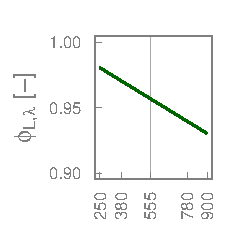
\includegraphics[width=\maxwidth]{figure/phi_L_lambda_vs_lambda-1} 

\end{knitrout}
      \label{fig:phi_light_graph}
    \end{subfigure}
    % add desired spacing between images (e.g., ~, \quad, \qquad, \hfill, etc.)
    % or a blank line to force the subfigure onto a new line.
    \begin{subfigure}[t]{0.74\textwidth}
\begin{knitrout}
\definecolor{shadecolor}{rgb}{0.969, 0.969, 0.969}\color{fgcolor}

\hfill{}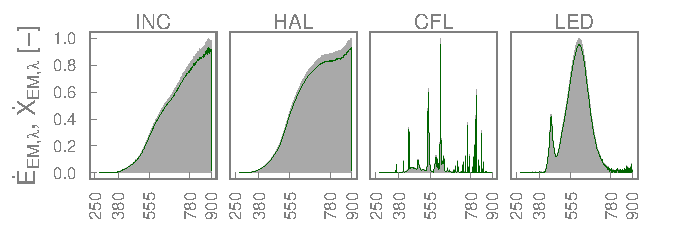
\includegraphics[width=\maxwidth]{figure/Energy_and_exergy_graph-1} 



\end{knitrout}
      \label{fig:lamp_exergy}
    \end{subfigure}
    \begin{subfigure}[t]{0.25\textwidth}
\begin{knitrout}
\definecolor{shadecolor}{rgb}{0.969, 0.969, 0.969}\color{fgcolor}
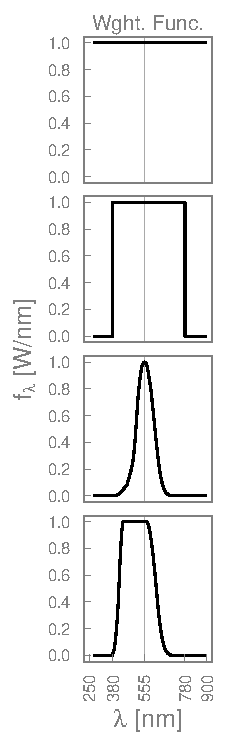
\includegraphics[width=\maxwidth]{figure/Weighting_Function_Graph_Energy-1} 

\end{knitrout}
        \label{fig:weighting_functions}
    \end{subfigure}
    % add desired spacing between images (e.g., ~, \quad, \qquad, \hfill, etc.)
    % or a blank line to force the subfigure onto a new line.
    \begin{subfigure}[t]{0.74\textwidth}
\begin{knitrout}
\definecolor{shadecolor}{rgb}{0.969, 0.969, 0.969}\color{fgcolor}

\hfill{}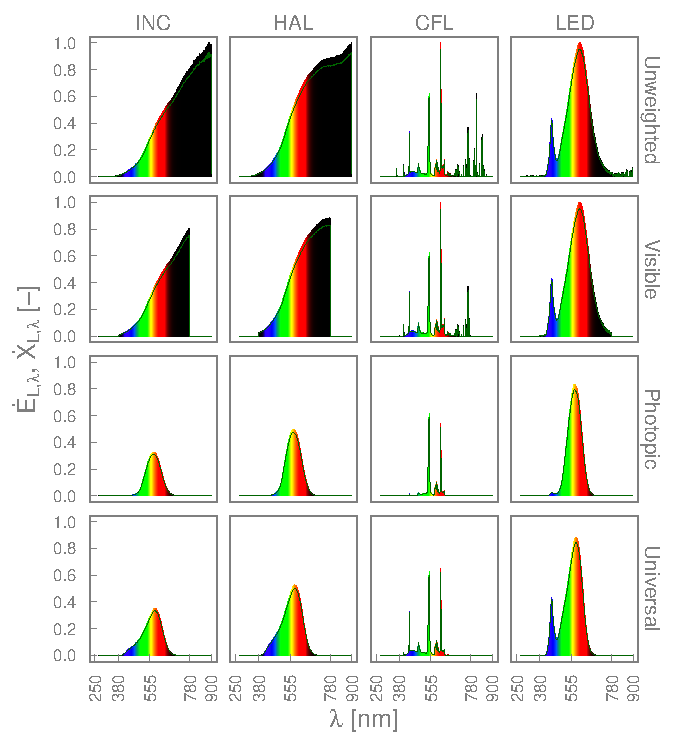
\includegraphics[width=\maxwidth]{figure/Responses_Graph_Energy-1} 



\end{knitrout}
        \label{fig:lamp_responses}
    \end{subfigure}%mdpi:it and its first mention crossed the first level title, please change position of it
    \caption{\hl{\textbf{Upper left}}: The spectral exergy-to-energy ratio of light~($\phi_{L,\lambda}$) 
                         from Equation~(\ref{eq:phi_L_lambda_shan_zhou}). 
             \mbox{\textbf{Top}: Gray regions} indicate spectral radiant power ($\dot{E}_{EM,\lambda}$)
                  for lamps in Table~\ref{tab:lamps}.
                  Dark green lines show spectral exergy ($\dot{X}_{EM,\lambda}$).
             \textbf{Left}: Spectral weighting functions ($f_\lambda$), as shown in Table~\ref{tab:wfs}.
             \mbox{\textbf{Lower right}}: Rainbow-colored regions indicate the human perception of color 
                          and the portion of light deemed valuable for human perception.
                          The tops of the rainbow regions give spectral light as energy~($\dot{E}_{L,\lambda}$).
                          \mbox{The dark} green lines show spectral light as exergy~($\dot{X}_{L,\lambda}$).
                          The spectral luminous power~($\Phi_{\lambda,pl}$) 
                          is shown in the ``Photopic'' row. 
             Peak spectral radiant power~($\dot{E}_{EM,\lambda}$) values are normalized to 1 for 
             for each lamp.}
	\label{fig:wfs_and_lamps}
\end{figure}
\unskip
\begin{table}[H]
\centering
\caption{Valuable energy efficiencies
                     ($\eta_{E,L,v}$, in \%) for each lamp
                     and each weighting function~($f_\lambda$),
                     \mbox{given by} Equation~(\ref{eq:eta_E_v_light}).
                     Note that for the incandescent (INC) and halogen (HAL) lamps, 
                     \mbox{the unweighted} energy efficiency~($\eta_{E,uw}$) is  
                     underestimated, because
                     the SPD data do not go beyond 899~nm, 
                     \mbox{despite INC} and HAL emission far into 
                     the infrared portion of the EM spectrum.} 
\label{tab:results_etas}
\begingroup\footnotesize
\begin{tabular}{ccccc}
  \toprule
 & \textbf{INC} & \textbf{HAL} & \textbf{CFL} & \textbf{LED} \\ 
  \midrule
Unweighted ($\eta_{E,uw}$) & 15.48 & 9.57 & 21.72 & 20.62 \\ 
  Vis. spectrum ($\eta_{E,vis}$) & 8.84 & 6.13 & 18.27 & 20.40 \\ 
  Photopic lum. ($\eta_{E,pl}$) & 2.06 & 1.61 & 9.27 & 10.25 \\ 
  Universal lum. ($\eta_{E,univ}$) & 2.69 & 2.14 & 13.37 & 13.65 \\ 
   \bottomrule
\end{tabular}
\endgroup
\end{table}
\unskip
\begin{table}[H]
\centering
\caption{Exergy-to-energy ratios~($\phi_L$) 
                     for each lamp 
                     and each weighting function ($f_{\lambda}$),
                     given by Equation~(\ref{eq:phi_L}).} 
\label{tab:results_phis}
\begingroup\footnotesize
\begin{tabular}{ccccc}
  \toprule
 & \textbf{INC} & \textbf{HAL} & \textbf{CFL} & \textbf{LED} \\ 
  \midrule
Unweighted ($\phi_{L,uw}$) & 0.943 & 0.944 & 0.953 & 0.954 \\ 
  Vis. spectrum ($\phi_{L,vis}$) & 0.949 & 0.949 & 0.955 & 0.954 \\ 
  Photopic lum. ($\phi_{L,pl}$) & 0.955 & 0.955 & 0.956 & 0.956 \\ 
  Universal lum. ($\phi_{L,univ}$) & 0.956 & 0.957 & 0.958 & 0.957 \\ 
   \bottomrule
\end{tabular}
\endgroup
\end{table}
\unskip
\begin{table}[H]
\centering
\caption{Valuable exergetic efficiencies
                     ($\eta_{X,L,v}$, in \%) for each lamp
                     and weighting function~($f_\lambda$),
                     \mbox{given by} Equation~(\ref{eq:eta_X_v_light}).
                     Similar to Table~\ref{tab:results_etas}, 
                     the unweighted exergetic efficiency~($\eta_{X,uw}$) is 
                     underestimated for the incandescent (INC) and halogen (HAL) lamps, because
                     the SPD data do not go beyond 899~nm, 
                     \mbox{despite INC} and HAL emission far into 
                     the infrared portion of the EM spectrum.} 
\label{tab:results_etasX}
\begingroup\footnotesize
\begin{tabular}{ccccc}
  \toprule
 & \textbf{INC} & \textbf{HAL} & \textbf{CFL} & \textbf{LED} \\ 
  \midrule
Unweighted ($\eta_{X,uw}$) & 14.59 & 9.04 & 20.69 & 19.67 \\ 
  Vis. spectrum ($\eta_{X,vis}$) & 8.38 & 5.82 & 17.45 & 19.47 \\ 
  Photopic lum. ($\eta_{X,pl}$) & 1.97 & 1.54 & 8.86 & 9.79 \\ 
  Universal lum. ($\eta_{X,univ}$) & 2.58 & 2.05 & 12.81 & 13.06 \\ 
   \bottomrule
\end{tabular}
\endgroup
\end{table}
%++++++++++++++++++++++++++++++
\subsection{Luminous Weighting Functions ($f_\lambda$)}
\label{sec:results_weighting_functions}
%++++++++++++++++++++++++++++++

The four luminous weighting functions 
discussed in Section~\ref{sec:weighting_functions} and Table~\ref{tab:wfs}
are shown on the left side of Figure~\ref{fig:wfs_and_lamps}.


%++++++++++++++++++++++++++++++
\subsection{Radiant Power ($\dot{E}_{EM,\lambda}$ and $\dot{X}_{EM,\lambda}$)}
\label{sec:results_radiant_power}
%++++++++++++++++++++++++++++++

The four graphs at the top of Figure~\ref{fig:wfs_and_lamps}
show normalized spectral radiant power ($\dot{E}_{EM,\lambda}$) 
at the top of the gray region for each lamp.
Applying Equation~(\ref{eq:phi_L_lambda_shan_zhou}) 
to the four lamps identified in Section~\ref{sec:lamps}
gives spectral radiant power in exergy terms ($\dot{X}_{EM,\lambda}$),
shown by the dark green line.
The areas of the gray regions ($\dot{E}_{EM}$) are given by Equation~(\ref{eq:emissive_power}).
The areas beneath the dark green lines in all graphs are the exergy of light~($\dot{X}_L$), 
given by Equation~(\ref{eq:X_dot_L}).

Note that exergy (dark green line) is very close to energy (top of the gray regions)
for all lamps, because
the exergy-to-energy ratio ($\phi_{L,\lambda}$) is always close to~1 for EM wavelengths relevant to light.
The difference between energy and exergy is greatest in the upper right of the graphs where both
%
\begin{enumerate*}[label={(\alph*)}]

  \item emission is greater and

  \item wavelength is longer.

\end{enumerate*}


%++++++++++++++++++++++++++++++
\subsection{Luminous Power ($\dot{E}_{L,\lambda}$ and $\dot{X}_{L,\lambda}$)}
\label{sec:results_luminous_power}
%++++++++++++++++++++++++++++++

Figure~\ref{fig:wfs_and_lamps} provides visual representation of the spectral energy and exergy of light
for the four lamps and four weighting functions of 
Sections~\ref{sec:weighting_functions} and~\ref{sec:lamps}
and Tables~\ref{tab:wfs} and~\ref{tab:lamps}, respectively.
\mbox{Each rainbow} colored region shows the energy content of light (spectral luminous power) and
is the spectral product of its row's weighting function and its column's lamp SPD.
The areas of the rainbow colored regions ($\dot{E}_L$) are given by Equation~(\ref{eq:L_dot_5}).
The areas beneath the dark green lines ($\dot{X}_L$) are given by 
Equation~(\ref{eq:X_dot_L}).


%++++++++++++++++++++++++++++++
\subsection{Energy Efficiencies ($\eta_{E,L,v}$)}
\label{sec:results_energy_efficiencies}
%++++++++++++++++++++++++++++++

Valuable energy efficiencies~($\eta_{E,L,v}$) of the various combinations of weighting functions and lamps
are shown in Table~\ref{tab:results_etas}.
Note that when a luminous weighting function is specified,
the lighting~($L$) and valuable~($v$) subscripts are implied and replaced by the weighting function specifier.
(E.g., \mbox{the valuable~($v$)} energy~($E$) efficiency~($\eta$) of light~($L$) 
using the visible luminous weighting function~($vis$),
$\eta_{E,L,v,vis}$, is written unambiguously as $\eta_{E,vis}$
for simplicity.)

% latex table generated in R 4.0.2 by xtable 1.8-4 package
%DIF <  Thu Sep 24 14:40:15 2020
%DIF >  Sun Oct 11 16:20:05 2020




%++++++++++++++++++++++++++++++
\subsection{Exergy-To-Energy Ratio ($\phi_L$)}
\label{sec:results_phi_L}
%++++++++++++++++++++++++++++++

Exergy-to-energy ratios~($\phi_{L}$) of the various combinations of weighting functions and lamps
are shown in Table~\ref{tab:results_phis}.

% latex table generated in R 4.0.2 by xtable 1.8-4 package
%DIF <  Thu Sep 24 14:40:17 2020
%DIF >  Sun Oct 11 16:20:06 2020




%++++++++++++++++++++++++++++++
\subsection{Exergetic Efficiencies ($\eta_{X,L,v}$)}
\label{sec:results_exergy_efficiencies}
%++++++++++++++++++++++++++++++
Valuable exergetic efficiencies~($\eta_{X,L,v}$) of the various combinations of weighting functions and lamps
are shown in Table~\ref{tab:results_etasX}.

% latex table generated in R 4.0.2 by xtable 1.8-4 package
%DIF <  Thu Sep 24 14:40:18 2020
%DIF >  Sun Oct 11 16:20:08 2020




%%%%%%%%%%%%%%%%%%%%%%%%%%%%%%%%%%%%%%%%%%%%%%%%%%%%%%%%%%%%%%
\section{Discussion}
\label{sec:discussion}
%%%%%%%%%%%%%%%%%%%%%%%%%%%%%%%%%%%%%%%%%%%%%%%%%%%%%%%%%%%%%%


%++++++++++++++++++++++++++++++
\subsection{Comparison between Conventional and Exact Methods
            to Calculating Exergetic Efficiency~($\eta_{X,L,v}$)}
\label{sec:compwithSEA}
%++++++++++++++++++++++++++++++

The exact method for calculating the exergetic efficiency of lamps
presented in Section~\ref{sec:light_efficiency}
differs from the conventional method 
used in the societal exergy analysis community (Section~\ref{sec:conventional_method}).
\mbox{This section}
%
\begin{enumerate*}[label={(\alph*)}]

  \item adds detail to the conventional method and

  \item evaluates the conventional method relative to the exact method,
        leading to three implications for societal exergy analysis
        (Section~\ref{sec:implications_for_sea}).

\end{enumerate*}


%------------------------------
\subsubsection{Conventional and Exact Methods} 
\label{sec:previous_approach}
%------------------------------

The conventional method (Section~\ref{sec:conventional_method}) 
estimates the valuable exergetic efficiency of lighting by the quotient of
the theoretical minimum rate of energy required to emit one lumen and
the actual rate of energy used to emit one lumen 
for a given lamp. 
The minimum and actual energy rates are obtained 
by inverting luminous efficacies.
For a lamp, the quotient is between the lamp's luminous efficacy~($K$)
and the maximum luminous efficacy~($K_{max}$).
Thus, 
\begin{equation} \label{eq:K_over_e_max}
  \eta_{X,L,v} \approx \frac{\; \; \frac{1}{K_{max}} \; \; }{\frac{1}{K}}
       = \frac{K}{K_{max}} \; ,
\end{equation}
% 
a restating of Equation~(\ref{eq:eta_eqn}).

Equation~(\ref{eq:lum_effic_def}) shows that 
the luminous efficacy of a lamp~($K$) is equal to the quotient
of the luminous power ($\Phi_{pl}$, Equation~(\ref{eq:lumen})), expressed in lm, and
the electricity consumption rate of the device
($\dot{W}_{elect,1}$ in Figure~\ref{fig:lamp}), expressed in W.
Substituting Equation~(\ref{eq:lum_effic_def}) into Equation~(\ref{eq:K_over_e_max}) restates
(with reference to Figure~\ref{fig:lamp})
valuable exergetic efficiency for the conventional method:
\begin{equation} \label{eq:prev_eta_X_v_light}
  \eta_{X,L,v} \approx \frac{ \; \; \frac{(683 \text{ lm/W}) \int V_\lambda \dot{E}_{EM,\lambda,3} \,
          \mathrm{d}\lambda}{\dot{W}_{elect,1}} \; \;}{K_{max}} \; .
\end{equation}

With recent advances in the fields of radiation thermodynamics and photometry
(Section~\ref{sec:phi_light}),
\mbox{it is} now possible to determine the energy and exergy of light exactly, 
thereby relieving societal exergy practitioners
of the need to estimate exergetic efficiency
by the quotient of
the minimum energy required to produce a lumen and
the actual energy required to produce a lumen.
Thus, we can evaluate the conventional method in light of recent advances, 
using exergetic efficiency~($\eta_{X,L,v}$) as the point \mbox{of comparison}.

Comparing Equation~(\ref{eq:prev_eta_X_v_light}) (the conventional method)
to Equation~(\ref{eq:eta_X_v_light}) (the exact method)
reveals that the conventional method for calculating the exergetic efficiency of lighting
is correct under the following conditions only:
%
\begin{enumerate}[leftmargin=8mm,labelsep=3mm] 

  \item[(1)] the maximum luminous efficacy ($K_{max}$) is taken to be 683~lm/W, 

  \item[(2)] $\phi_{L,\lambda} = 1$ for all wavelengths, and

  \item[(3)] the spectral luminous weighting function~($f_\lambda$) is taken to be
        the photopic luminous weighting function ($V_\lambda$).

\end{enumerate}

Condition~(a) shows that the correct assumption for maximum luminous efficacy 
in the conventional method 
is $K_{max} = 683 \text{ lm/W}$.
Any other assumption is a mistake.
The assumption in condition~(b) is incorrect;
the exergy-to-energy ratio for light~($\phi_{L,\lambda}$) is not 1
(as shown in Equation~(\ref{eq:phi_L_lambda_shan_zhou})), but the conventional method assumes it is.
Condition~(c) highlights an unfortunate requirement of the conventional method, 
one that is lifted by the exact method.

When $K_{max}$ is equal to 683~lm/W and
the weighting function is taken to be the photopic luminous weighting function~($V_\lambda$),
as they should for the conventional method,
Equation~(\ref{eq:prev_eta_X_v_light}) simplifies to 
\begin{equation} \label{eq:prev_eta_X_v_light_final}
  \eta_{X,L,v} \approx \frac{\int V_\lambda \dot{E}_{EM,\lambda,3} \mathrm{d}\lambda}{\dot{W}_{elect,1}}\; .
\end{equation}

So the conventional method's estimate 
of a lamp's valuable exergetic efficiency
(Equation~(\ref{eq:K_over_e_max})) 
reduces to Equation~(\ref{eq:prev_eta_X_v_light_final}), 
which is the same as Equation~(\ref{eq:eta_E_v_light}),
the valuable energy efficiency of a lamp, 
\mbox{if $f_\lambda = V_\lambda$}.
That is to say, one interpretation of the conventional method
is that it incorrectly 
assumes the \emph{exergetic} efficiency of a lamp
to be its \emph{energy} efficiency.


%------------------------------
\subsubsection{Implications for Societal Exergy Analysis} 
\label{sec:implications_for_sea}
%------------------------------



The above comparison between the conventional method (Section~\ref{sec:previous_approach}) and
the exact method (Section~\ref{sec:framework})
raises three implications for societal exergy analysis.
First, with the conventional method, 
the practitioner is required to select a value for maximum luminous efficacy ($K_{max}$), 
the denominator of Equation~(\ref{eq:K_over_e_max}).
The choice of $K_{max}$ can make a significant difference to the results.
The correct value for $K_{max}$ is 683~lm/W,
as discussed in Section~\ref{sec:previous_approach}.
We showed in Section~\ref{sec:conventional_method} that
some practitioners have mistakenly, we now know, taken $K_{max}$ to be 
220~lm/W or 400~lm/W,
thereby overestimating exergetic efficiency of lighting~($\eta_{X,L,v}$)
with the conventional method
by a factor of
$\frac{683 \text{ lm/W}}{220 \text{ lm/W}} 
  = 3.1$
or
$\frac{683 \text{ lm/W}}{400 \text{ lm/W}} 
  = 1.7$,
respectively.

Second, to obtain the correct exergetic efficiency of lighting, 
practitioners must reject the conventional method assumption that $\phi_{L,\lambda} = 1$.
Recent progress in the exergy of radiation enables this rejection, 
following the methods of Section~\ref{sec:phi_light}.
Specifically, the spectral exergy-to-energy ratio of light ($\phi_{L,\lambda}$)
of Equation~(\ref{eq:phi_L_lambda_shan_zhou}) and Figure~\ref{fig:wfs_and_lamps} should be used.
We note, however, that $\phi_{L,\lambda}$ is close to~1 for all wavelengths of interest to illumination.
Happily, the conventional method was not far wrong.

Third, in the conventional method, 
the practitioner is required to use the photopic luminous weighting function~($V_\lambda$)
for the spectral luminous weighting function~($f_\lambda$).
However, it is not certain that the photopic luminous weighting function
is the best choice.
In fact, we later recommend replacing the photopic luminous weighting function~($V_\lambda$)
by the universal luminous weighting function~($U_\lambda$).
(See Section~\ref{sec:reccuniv}).


%++++++++++++++++++++++++++++++
\subsection{Recommendations}
\label{sec:recommendations}
%++++++++++++++++++++++++++++++

We provide three recommendations for societal exergy practitioners:
%
\begin{enumerate*}[label={(\alph*)}]

  \item use the exact method of Section~\ref{sec:methods} when possible, 
        i.e., when SPD data are available for a lamp or lamp technology, 

  \item use the universal luminous weighting function~($U_\lambda$) always, and

  \item use an approximate method when luminous efficacy~($K$) data are available, but
        SPD data are not.

\end{enumerate*}


%------------------------------
\subsubsection{Recommendation for the Exact Method} 
\label{sec:recommend_exact_method}
%------------------------------

Our first recommendation is for use of the 
exact method~(Section~\ref{sec:light_efficiency})
for determining the valuable exergetic efficiency of lamps~($\eta_{X,L,v}$)
when SPD data are available.
The exact method provides the following benefits over the conventional method:
%
\begin{enumerate}[leftmargin=8mm,labelsep=3mm] 


  \item[(a)] it is free of any assumptions for the maximum luminous efficacy ($K_{max}$),

  \item[(b)] it uses a non-unity spectral exergy-to-energy ratio, no longer assuming $\phi_{L,\lambda} = 1$, and 

  \item[(c)] it allows choices for the spectral luminous weighting function~($f_\lambda$), 
        no longer requiring $f_\lambda = V_\lambda$, 
        thereby enabling our second recommendation, 
        namely use of the universal luminous weighting function ($U_\lambda$).

\end{enumerate}


%------------------------------
\subsubsection{Recommendation for the Universal Luminous Weighting Function~($U_\lambda$)} 
\label{sec:reccuniv}
%------------------------------

We recognize that the choice of spectral weighting function~($f_\lambda$)
remains contentious~\cite{Delgado-Bonal:2017aa, Pattison2018LEDphotons, Rea2018, Royer2016}.
That said, we suggest that the choice of weighting function \DIFdelbegin %DIFDELCMD < \del{ ($f_\lambda$)} %%%
\DIFdelend in societal exergy analysis
should be appropriate for each lamp's application.
Our second recommendation is for use of
the universal luminous weighting function~($U_\lambda$) in societal exergy analysis
when the purpose of lamps \mbox{is illumination}.

For the application of illumination, 
we note that human perception of light and color diminishes rapidly above 700~nm,
as shown by Figure~\ref{fig:wfs_and_lamps}.
This decline in human eye sensitivity toward the infra-red region
is captured well by the photopic luminous weighting function~($V_\lambda$).

However, it is also known that short wavelength EM radiation (bluer light)
provides physiological benefits, such as
the suppression of melanopsin and 
the regulation of circadian rhythms~\citep{Pattison2018LEDphotons}.
\mbox{The photopic} luminous weighting function~($V_\lambda$) does not
capture the importance of short wavelength EM radiation, 
attenuating human perception nearly equally in the blue and red regions
of the visible spectrum.

Societal exergy analysis implicitly adopts the photopic luminous weighting function~($V_\lambda$)
when it applies the conventional method for calculating the exergetic efficiency of lighting.
(See Section~\ref{sec:previous_approach}).
For lamps whose purpose is illumination, 
we believe that, instead, the universal luminous weighting function ($U_\lambda$)
is most appropriate.
(See also \citet{Rea2018}).
We provide three arguments in support of this recommendation.

First, 
the universal luminous weighting function~($U_\lambda$)
accounts for the sensitivity of all five types of light receptors in the human eye,
whereas the photopic luminous weighting function~($V_\lambda$) does not.

Second,
to obtain the benefits of blue light, 
many lamps are designed with a blue spike 
in the region of 480~nm, 
the peak of the melanopsin suppression action spectrum \cite{lucas2014}.
(For example, \mbox{see the} blue spike in the SPD~($\dot{E}_{EM,\lambda}$)
for the LED lamp in Figure~\ref{fig:wfs_and_lamps}).
The universal luminous weighting function~($U_\lambda$)
correctly includes the energy or exergy of blue spikes
in the numerator of efficiency calculations,
thereby correctly elevating the efficiency of lamps that contain a blue spike
compared to the photopic luminous weighting function.

Third, 
manufacturers who design lamps with blue spikes
do not get credit for their efforts, because 
the industry-standard measure of lighting efficiency,
luminous efficacy~($K$), 
uses the photopic luminous weighting function~($V_\lambda$). 
This state of affairs could encourage lamp manufacturers to reduce short wavelength
output of lamps, even when short wavelength EM radiation would 
provide physiological benefits.
Adopting the universal luminous weighting function will alleviate 
the incentive for manufacturers to minimize the size of blue spikes,
providing a greater range of options for the design 
of SPDs for lamps that produce white light.

The conventional method for estimating lamp efficiency
is bound by the use of the photopic luminous weighting function.
However, a switch away from the photopic luminous weighting function~($V_\lambda$)
toward the universal luminous weighting function~($U_\lambda$) is
made possible by the exact method described in Section~\ref{sec:framework},
so long as SPD data are available.
In the absence of SPD data, 
\mbox{we recommend} an approximate method, 
as set out in the next section.


%------------------------------
\subsubsection{Recommendation for an Approximate Method} 
\label{sec:approximate_method}
%------------------------------

Section~\ref{sec:previous_approach} shows that the conventional method does not require SPD information, 
but it produces energy efficiency (instead of exergetic efficiency)
while requiring the use of photopic luminous weighting function~($\eta_{E,pl}$).
In contrast, we recommend that,
in the absence of SPD data,
societal exergy practitioners
calculate exergetic efficiency 
with the universal luminous weighting function~($\eta_{X,univ}$).
Thus, our third recommendation is for an approximate method to determine 
the valuable exergetic efficiency of lamps~($\eta_{X,L,v}$)
when SPD data are not available
but luminous efficacy data~($K$) are.
Results from the exact method provide guidance 
for development of an approximate method.

We suggest the following two-step process:  
using the conventional method as a starting point,
%
\begin{enumerate}

  \item move from valuable energy efficiency~($\eta_{E,pl}$)
        to valuable exergetic efficiency ($\eta_{X,pl}$)
        using an average exergy-to-energy ratio~($\bar{\phi}_{L,pl}$) and 

  \item move from valuable exergetic efficiency determined with the photopic luminous weighting function~($\eta_{X,pl}$)
        to valuable exergetic efficiency determined with the universal luminous weighting function~($\eta_{X,univ}$)
        using an average ratio between those efficiencies,
        the average photopic-to-universal conversion factor~($\gammaratavg{}$).

\end{enumerate}









%..............................
\paragraph{\emph{\hl{Estimating} the average exergy-to-energy ratio~($\bar{\phi}_{L,pl}$)}} %mdpi:please confirm whether it should be changed to 4th title
%..............................

We calculated the exergy-to-energy ratio for a sample of lamps from the LSPDD \cite{aube2013}
using Equation~(\ref{eq:phi_L}) with $f_\lambda = V_\lambda$. 
(The sample consists of 45 lamp SPDs representing six technologies: 
INC, HAL, CFL, LED, HPS (high pressure sodium), and MH (metal halide).
The average value for the exergy-to-energy ratio is
$\bar{\phi}_{L,pl} = 0.956$ 
with a remarkably small standard deviation of $\sigma_{\phi_{L,pl}} = 0.00037$. Table~\ref{tab:mean_phi_p2_by_lamp_type} shows 
statistics for the exergy-to-energy ratio~($\bar{\phi}_{L,pl}$)
by lighting technology.

%DIF >  latex table generated in R 4.0.2 by xtable 1.8-4 package
%DIF >  Sun Oct 11 16:20:09 2020
\begin{table}[H]
\centering
\caption{The mean~($\bar{\phi}_{L,pl}$),
                     standard deviation~($\sigma_{\phi_{L,pl}}$), and 
                     sample size~($n$)
                     of the exergy-to-energy ratio when using
                     the photopic luminous weighting function,
                     by lighting technology.} 
\label{tab:mean_phi_p2_by_lamp_type}
\begingroup\footnotesize
\begin{tabular}{ccccccc}
  \toprule
 & \textbf{INC} & \textbf{HAL} & \textbf{CFL} & \textbf{LED} & \textbf{MH} & \textbf{HPS} \\ 
  \midrule
\DIFaddendFL $\bar{\phi}_{L,pl}$  & 0.955 & 0.956 &0.956 & 0.956 & 0.956 & 0.955 \\ 
 $\sigma_{\phi_{L,pl}}$ & 0.000148 &0.000097 & 0.000419 & 0.000361 & 0.000196 &  \\ 
 $n$ & 11 & 10 & 10 & 10& 3& 1\\ 
   \bottomrule
\end{tabular}
\endgroup
\end{table}
\DIFaddend 



%..............................
\paragraph{\emph{\hl{Estimating} the average photopic-to-universal conversion factor~($\gammaratavg{}$)}}
%..............................

Similarly, we obtained $\gammarat{}$ for each lamp~($i$) by taking the quotient of efficiencies:
\begin{equation} \label{eq:conversionuniversal}
  \gammarat{}_{,i} = \frac{\eta_{X,univ,i}}{\eta_{X,pl,i}} \; .
\end{equation}

Because a greater proportion of each SPD is considered to be light
by the universal luminous weighting function~($U_\lambda$)
compared to the photopic luminous weighting function~($V_\lambda$), 
$\gammarat{}$ is expected to be greater than 1.
The average value of the photopic-to-universal factor across our population of lamps 
was $\gammaratavg{} = 1.36$,
with a small standard deviation of $\sigma_{\gammarat{}} = 0.095$. Table~\ref{tab:conversionfactors} shows 
statistics for the photopic-to-universal factor~($\gammaratavg{}$)
by lighting technology.

%DIF >  latex table generated in R 4.0.2 by xtable 1.8-4 package
%DIF >  Sun Oct 11 16:20:09 2020
\begin{table}[H]
\centering
\caption{The mean~($\bar{\gamma}_{pl\rightarrow{}univ}$),
                     standard deviation~($\sigma_{\gamma_{pl\rightarrow{}univ}}$), and 
                     sample size~($n$)
                     of the photopic-to-universal factor,
                     by lighting technology.} 
\label{tab:conversionfactors}
\begingroup\footnotesize
\begin{tabular}{ccccccc}
  \toprule
 & \textbf{INC} & \textbf{HAL} & \textbf{CFL} & \textbf{LED} & \textbf{MH} & \textbf{HPS} \\ 
  \midrule
\DIFaddendFL $\gammaratavg{}$ \DIFdelbeginFL & 1.32 & 1.36 & {1.38 }& 1.34 & 1.51 & 1.19 \\ 
  {$\sigma_{\gammarat}$ }&0.029 & {0.031 }& {0.138 }& {0.097 }& {0.048 }&  \\ 
  {$n$ }&{11 }& {10 }& {10 }& {10 }& {3 }& {1 }\\ 
   \bottomrule
\end{tabular}
\endgroup
\end{table}
\DIFaddend 



%..............................
\paragraph{\emph{\hl{Implementing} the approximate method}}
%..............................

The approximate method for determining the valuable exergetic efficiency of a lamp
is implemented by the following equation
\begin{equation} \label{eq:approximate}
  \eta_{X,univ} \approx \bar{\phi}_{L,pl} \, \gammaratavg{} \, \frac{K}{683 \text{ lm/W}} \; ,
\end{equation}
%
which is a modification of Equation~(\ref{eq:K_over_e_max})
that approximates the move from energy to exergy
assuming the photopic luminous weighting function (via $\bar{\phi}_{L,pl}$)
and the move from the photopic luminous weighting function to the universal luminous weighting function
in the exergy space (via $\gammaratavg{}$).

When the lamp technology is unknown, overall average values can be used
for $\bar{\phi}_{L,pl}$ and $\gammaratavg{}$:
\begin{equation} \label{eq:approximate_unknown_tech}
  \eta_{X,univ} \approx (0.956) 
                        (1.36)
                        \frac{K}{683 \text{ lm/W}} 
                      = 1.30 \,
                        \frac{K}{683 \text{ lm/W}} \; .
\end{equation}

If the lamp technology is known, 
$\bar{\phi}_{L,pl}$ and $\gammaratavg{}$ values 
from Tables~\ref{tab:mean_phi_p2_by_lamp_type} and~\ref{tab:conversionfactors} 
could be used instead of the averages across all technologies shown in Equation~(\ref{eq:approximate_unknown_tech}).

Table~\ref{tab:threemethods} summarizes 
the valuable exergetic efficiency 
for the four representative lamps (INC, HAL, CFL, LED) and
the three methods (conventional, exact, and approximate).


% latex table generated in R 4.0.2 by xtable 1.8-4 package
%DIF <  Thu Sep 24 14:40:19 2020
%DIF >  Sun Oct 11 16:20:09 2020
\begin{table}[H]
\centering
\caption{Valuable exergetic efficiencies (in \%)
                     for each of the three methods
                     (conventional, exact, \mbox{and approximate}) and
                     each of the four example lamps
                     (INC, HAL, CFL, LED).
                     Note that the conventional method row is the same as
                     row 3 of Table~\ref{tab:results_etas}.
                     The exact method row is the same as
                     row 4 of Table~\ref{tab:results_etasX}.
                     The approximate method row uses
                     the values for $\bar{\phi}_{L,pl}$ and $\gammaratavg{}$ shown
                     in Equation~(\ref{eq:approximate_unknown_tech}).} 
\label{tab:threemethods}
\begingroup\footnotesize
\begin{tabular}{ccccc}
  \toprule
 & \textbf{INC} & \textbf{HAL} & \textbf{CFL} & \textbf{LED} \\ 
  \midrule
Conventional method ($\eta_{E,pl}$) & 2.06 & 1.61 & 9.27 & 10.25 \\ 
  Exact method ($\eta_{X,univ}$) & 2.58 & 2.05 & 12.81 & 13.06 \\ 
  Approximate method (Equation~\eqref{eq:approximate_unknown_tech}) & 2.68 & 2.09 & 12.03 & 13.30 \\ 
   \bottomrule
\end{tabular}
\endgroup
\end{table}



%++++++++++++++++++++++++++++++
\subsection{Aggregate Lighting Efficiencies}
\label{sec:AggEfficiencies}
%++++++++++++++++++++++++++++++

Societal exergy analyses are normally conducted at the sectoral or economy-wide scale, 
\mbox{so practitioners} must weight per-lamp-technology efficiencies
by each technology's usage fraction.
\mbox{Two types} of data are needed for a given period of interest, typically a year:
%
\begin{enumerate*}[label={(\alph*)}]

  \item valuable exergetic efficiency data for each lamp technology~($\eta_{X,univ,i}$) and

  \item proportion of lighting electricity consumption by lamp technology~($\theta_i$),

\end{enumerate*}
%
where $i$ denotes individual lighting technologies.

Item (a) is the result of applying the exact method to each lamp technology
but depends on the availability of representative SPDs for each technology,
which are not often known.
Instead, the most common measure of lighting efficiency 
reported for a lamp technology is the luminous efficacy~($K$).
Therefore, to develop an aggregate measure of lighting efficiency, 
luminous efficacies must be converted 
into valuable exergetic efficiencies by the approximate method.
(See Section~\ref{sec:approximate_method}).

Data for item~(b) are in the form of the fraction of lighting electricity consumed by each lamp technology.
Such data (and luminous efficacy values, $K_i$)
can be obtained from the US DOE's Lighting Market Characterization reports \citep{DOE2002, DOE2012, DOE2017}
for the USA for the following lamp technologies: incandescent, halogen, compact fluorescent,
linear fluorescent, high intensity discharge, LED, and other.

When SPDs are available, the exact method can be used to determine the 
valuable exergetic efficiency of each lighting technology~($i$), and
the aggregate valuable exergetic lighting efficiency for a particular year can be found by
\begin{equation} \label{eq:agg_eta}
  \eta_{X,univ,agg} = \sum \limits_{i} \theta_{i} \, \eta_{X,univ,i} \; .
\end{equation}
%

When SPDs are not available, the approximate method can be used as follows:
\begin{equation} \label{eq:agg_eta_K}
  \eta_{X,univ,agg} \approx \sum \limits_{i} \theta_{i} \, \bar{\phi}_{L,pl} \, \gammaratavg{} \, 
                            \frac{K_{i}}{683 \text{ lm/W}} \; .
\end{equation}


%%%%%%%%%%%%%%%%%%%%%%%%%%%%%%%%%%%%%%%%%%%%%%%%%%%%%%%%%%%%%%
\section{Summary and Future Work}
\label{sec:conclusions}
%%%%%%%%%%%%%%%%%%%%%%%%%%%%%%%%%%%%%%%%%%%%%%%%%%%%%%%%%%%%%%

% This section is not mandatory, but can be added to the manuscript if the discussion is unusually long or complex.

Several recent developments in the 
fields of radiation thermodynamics and photometry
(the spectral exergy-to-energy ratio, $\phi_{L,\lambda}$, and 
the photon effective temperature, $T_\lambda$) 
have enabled
a re-evaluation of the exergy of light and the exergetic efficiency of electric lamps
applicable to societal exergy analysis.
We built upon those advances to provide 
clear and rigorous definitions of the energy and exergy of light.
We developed a novel exact method for determining the exergetic efficiency of lamps
involving the 
spectral exergy-to-energy ratio~($\phi_{L,\lambda}$), 
a luminous weighting function~($f_\lambda$), \mbox{and 
broad-spectrum} lamp luminous power~($\dot{E}_{EM}$).
We showed that the exact method
%
\begin{enumerate*}[label={(\alph*)}]

  \item is free of any assumptions for the maximum luminous efficacy ($K_{max}$),

  \item uses a non-unity spectral exergy-to-energy ratio~($\phi_{L,\lambda}$), and

  \item allows choices for the spectral luminous weighting function ($f_\lambda$).

\end{enumerate*}
%
Items (a)--(c) are improvements over the conventional method.
The exact method requires the availability of a lamp's spectral power distribution.
For cases when a spectral power distribution is not available, 
\mbox{we developed} a novel approximate method,
involving surprisingly stable values 
of the exergy-to-energy ratio~($\phi_L$) and 
the photopic-to-universal conversion factor~($\gammarat{}$)
across lighting technologies.
Finally, we provided recommendations for societal exergy practitioners, namely to use
%
\begin{enumerate*}[label={(\alph*)}]

  \item the exact method when a lamp's spectral power distribution is available, 

  \item the universal luminous weighting weighting function~($U_\lambda$), and

  \item the approximate method when luminous efficacy is known
        but spectral power distribution is not.

\end{enumerate*}

Future work could include
%
\begin{enumerate*}[label={(\alph*)}]

	\item investigating additional lighting technologies to assess the stability of 
	      the average exergy-to-energy ratio~($\bar{\phi}_{L,pl}$) and 
	      the average photopic-to-universal conversion factor~($\gammaratavg{}$)
	      across lighting technologies,

  \item applying the exact method to understand the evolution
        of lighting technology relative to the maximum possible reductions 
        in lighting energy consumption~\citep{CullenPhD}
        (via gains in 
        lamp luminous efficacy~($K$) and valuable exergetic efficiency, $\eta_{X,L,v}$),

  \item understanding the effect of lamp ``waste'' heat on lamp efficiency
        (lamp heat is beneficial when it displaces energy for winter space heating but
        detrimental when it adds to summer cooling loads), and 

  \item pushing toward the services stage of the energy conversion chain
        to assess the effects of waste light 
        (caused by 
        excessive intensity, 
        lighting that falls on surfaces that do not require illumination, \mbox{or
        under-utilization} of light due to under-occupancy of spaces).

\end{enumerate*}




%%%%%%%%%%%%%%%%%%%%%%%%%%%%%%%%%%%%%%%%%%
\vspace{6pt} 


%%%%%%%%%%%%%%%%%%%%%%%%%%%%%%%%%%%%%%%%%%
%MDPI:this part is not mentioned in main text, please confirm
\supplementary{\hl{The following} are available online at \url{https://doi.org/10.5518/865}~\cite{heun2020}:
sources for the luminous efficacy values in Figure~\ref{fig:LuminousEfficacy_Graph}, 
sources for the weighting functions and SPDs displayed in Figure~\ref{fig:wfs_and_lamps}, 
instructions and R code for reproducing the metrics and figures in this paper, and
a blank excel workbook template in the required format 
for the insertion of spectral power distribution data by the user.}


%%%%%%%%%%%%%%%%%%%%%%%%%%%%%%%%%%%%%%%%%%
\authorcontributions{Conceptualization: M.K.H., Z.M., E.A., and P.E.B.; 
methodology: M.K.H., Z.M., and E.A.; 
software: M.K.H., Z.M., and E.A.; 
validation: M.K.H. and Z.M.; 
formal analysis: M.K.H., Z.M., and E.A.; 
investigation: M.K.H. and Z.M.; 
resources: M.K.H.; 
data curation: M.K.H. and Z.M.; 
writing--original draft preparation: M.K.H., Z.M., E.A., and P.E.B.; 
writing--review and editing: M.K.H., Z.M., E.A., and P.E.B.; 
visualization: M.K.H., Z.M., and E.A.; 
supervision: M.K.H. and P.E.B.; 
project administration: M.K.H. and P.E.B.; 
funding acquisition: P.E.B.
All authors have read and agreed to the published version of the manuscript.}


%%%%%%%%%%%%%%%%%%%%%%%%%%%%%%%%%%%%%%%%%%
\funding{Zeke Marshall's and Paul E. Brockway time was 
funded by the UK Research Council under EPSRC Fellowship award EP/R024254/1.
Emmanuel Aramendia's time was funded by the University of Leeds (School of Earth and Environment).
Matthew Kuperus Heun has no funding to declare.
}


%%%%%%%%%%%%%%%%%%%%%%%%%%%%%%%%%%%%%%%%%%
\acknowledgments{The authors thank
James D. Hooker for
  the use of data from the Museum of Electric Lamp Technology~\cite{hooker_2020}, 
Alfonso Delgado-Bonal for
  his advice on the state of the discourse regarding the exergy-to-energy ratio of light, 
Pedro J. Aphalo for
  his open-source software suite \texttt{r4phototbiology}~\cite{Aphalo2015}, 
Martin Aub\`{e} and Johanne Roby for
  the use of their Light Spectral Power Distribution Database (LSPDD)~\cite{aube2013}, 
Andrew Stockman and other members of the Colour and Vision Research 
  % Laboratory for data for the photopic luminous weighting function~\cite{CVRL2008},
  Laboratory for their open-source database 
  from which we obtained data for the photopic luminous weighting function~\cite{CVRL2008},
Mark S. Rea and Andrew Bierman for
  the use of the universal luminous weighting function~\cite{Rea2018}, and
Micheal Royer for
  his advice regarding photometric data.
}


%%%%%%%%%%%%%%%%%%%%%%%%%%%%%%%%%%%%%%%%%%
\conflictsofinterest{The authors declare no conflicts of interest. 
The funders had no role in the design of the study; 
in the collection, analyses, or interpretation of data; 
in the writing of the manuscript; or 
in the decision to publish the results.} 


%%%%%%%%%%%%%%%%%%%%%%%%%%%%%%%%%%%%%%%%%%%%%%%%%%%%%%%%%%%%%%
\section*{Nomenclature}
\label{sec:nomenclature}
%%%%%%%%%%%%%%%%%%%%%%%%%%%%%%%%%%%%%%%%%%%%%%%%%%%%%%%%%%%%%%

%MDPI:we changed Table~\ref{tab:long_nomenclature} shows nomenclature, including symbols, Greek letters, subscripts, and abbreviations. Note that an overdot (e.g., $\dot{x}$) indicates a steady state rate, not a first derivative with respect to time to  The following symbols, greek letters, subscripts, and abbreviations are used in this manuscript:, and i deleted caption of the table, please confirm

\noindent{The following symbols, greek letters, subscripts, and abbreviations are used in this manuscript:}

%\begin{center}
%\begin{longtable}{ll}%mdpi:please delete it
%\caption{\hl{Nomenclature.}} \label{tab:long_nomenclature} \\

\vspace{6pt}
 \noindent
\begin{tabular}{ll}
Symbol & Meaning [example units] \\ 
%\midrule 
%\endfirsthead
%
%%\multicolumn{2}{c}{\small {\bfseries \tablename\ \thetable{}, continued.} Nomenclature.} \\
%%\toprule 
%%Symbol & Meaning [example units] \\ 
%%\midrule 
%\endhead
%
%%\bottomrule
%%\multicolumn{2}{r}{Continues on next page} \\ 
%\endfoot
%
%%\bottomrule
%\endlastfoot
  $c$ & speed of light, $3 \times 10^8 \text{ m/s}$ \\
  $c_3$ & constant for photon effective temperature, $5.33016 \times 10^{-3} \text{ m-K}$ \\
  $E$ & energy [J] \\
  $\dot{E}$ & energy rate [W] \\
  $f_\lambda$ & spectral weighting function [--] \\
  $h$ & Planck's constant, $6.626 \times 10^{-34} \text{ J-s}$ \\
  $K$ & luminous efficacy [lm/W] \\
  $K_{max}$ & luminous efficacy of a perfect light source at 555~nm [lm/W] \\
  $\dot{Q}$ & heat rate [W] \\
  $T$ & temperature [K] \\
  $T_\lambda$ & effective temperature of light photons [K] \\
  $U_\lambda$ & universal luminous weighting function [--] \\
  $V_\lambda$ & photopic luminous weighting function [--] \\
  $\dot{W}$ & work rate [W] \\
  $\dot{X}$ & exergy rate [W] \\
%
%\midrule
\multicolumn{2}{l}{\emph{Greek}} \\ 
%
  $\eta$ & efficiency [--] \\
  $\gammarat$ & photopic-to-universal scale factor for $\eta_{X,L,v}$ [--] \\
  $\gammaratavg$ & average photopic-to-universal scale factor for $\eta_{X,L,v}$ [--] \\
  $\lambda$ & wavelength of EM radiation [nm] \\
  $\mu$ & scale factor between relative and absolute intensity [--] \\
  $\nu$ & frequency of EM radiation [1/s] \\
  $\Phi_{pl}$ & luminous power [lm] \\
  $\phi$ & exergy-to-energy ratio [--] \\
  $\bar{\phi}$ & average exergy-to-energy ratio [--] \\
  $\sigma$ & standard deviation \\
%
%\midrule
\multicolumn{2}{l}{\emph{Subscripts}} \\ 
%
  $0$ & ambient temperature or absorber temperature \\
  $1$ & emitter temperature \\
  $agg$ & aggregate \\
  $C$ & Carnot efficiency \\
  $D$ & exergy destroyed \\
  $elect$ & electricity \\
  $E\!M$ & electro-magnetic \\
  $E$ & energy \\
  $i$ & index for lamp type or lamp technology \\
  $\lambda$ & spectral (a function of wavelength) \\
  $L$ & light \\
  $max$ & maximum luminous efficacy \\

  $N$ & non-light EM radiation \\
  $pl$ & denotes the application of the photopic luminosity function ($V_{\lambda}$) \\
  $Q$ & heat \\
\end{tabular}

\noindent
\begin{tabular}{ll}
  $rel$ & relative intensity \\
  $sys$ & system operating temperature \\
  $univ$ & denotes the application of the universal weighting function~($U_\lambda$) \\
  $uw$ & unweighted \\
  $v$ & valuable \\
  $vis$ & visible spectrum or visible weighting function \\
  $W$ & work \\
  $X$ & exergy \\
%
%\midrule
\multicolumn{2}{l}{\emph{Abbreviations}} \\ 
%
  CFL & compact fluorescent light \\
  CIE & Commission Internationale de l\textquotesingle{}Eclairage \\
  CMF & color matching function \\
  DOE & Department of Energy \\
  EM & electromagnetic \\
  HAL & halogen \\
  HPS & high-pressure sodium \\
  INC & incandescent \\
  ipRGCs & intrinsically photosensitive retinal ganglion cells \\
  LED & light-emitting diode \\
  LSPDD & Light Spectral Power Distribution Database \\
  MH & metal halide \\
  SPD & spectral power distribution \\
  UK & United Kingdom \\
  US, USA & United States of America \\
%%
%\end{longtable}
%\end{center}
\end{tabular}

%%%%%%%%%%%%%%%%%%%%%%%%%%%%%%%%%%%%%%%%%%
%% optional
%\appendixtitles{yes} 
%% Leave argument "no" 
%% if all appendix headings stay EMPTY
%% (then no dot is printed after "Appendix A").
%% If the appendix sections contain a heading then change the argument to "yes".
%
%
%%%%%%%%%%%%%%%%%%%%%%%%%%%%%%%%%%%%%%%%%%%
%\DIFdelbegin %DIFDELCMD < \appendix
%%DIFDELCMD < 
%
%%DIFDELCMD < %%%
%%DIF <  The appendix is an optional section that can contain 
%%DIF <  details and data supplemental to the main text. 
%%DIF <  For example, explanations of experimental details 
%%DIF <  that would disrupt the flow of the main text, but 
%%DIF <  nonetheless remain crucial to understanding and reproducing the research shown; 
%%DIF <  figures of replicates for experiments 
%%DIF <  of which representative data is shown in the main text 
%%DIF <  can be added here if brief, or as Supplementary data. 
%%DIF <  Mathematical proofs of results not central to the paper can be added as an appendix.
%%DIFDELCMD < 
%
%%DIFDELCMD < %%%
%%DIF < %%%%%%%%%%%%%%%%%%%%%%%%%%%%%%%%%%%%%%%%%%%%%%%%%%%%%%%%%%%%%
%%\section{Average exergy-to-energy ratio~($\bar{\phi}_{L,pl}$)
%%         and photopic-to-universal factor~($\gammaratavg$)
%%         by lighting technology}
%%DIFAUXCMD
%\addtocounter{section}{-1}%DIFAUXCMD
%%DIFDELCMD < \label{sec:non_light}
%%DIFDELCMD < %%%
%%DIF < %%%%%%%%%%%%%%%%%%%%%%%%%%%%%%%%%%%%%%%%%%%%%%%%%%%%%%%%%%%%%
%  %DIFDELCMD < 
%
%%DIFDELCMD < %%%
%%DIF <  All appendix sections must be cited in the main text. 
%%DIF <  In the appendixes, Figures, Tables, etc. should be labeled starting with `A', 
%%DIF <  e.g., Figure A1, Figure A2, etc. 
%%DIFDELCMD < 
%
%%DIFDELCMD < %%%
%\DIFdel{Table~\ref{tab:mean_phi_p2_by_lamp_type} shows 
%statistics for the exergy-to-energy ratio~($\bar{\phi}_{L,pl}$)
%by lighting technology.
%}%DIFDELCMD < 
%
%%DIFDELCMD < %%%
%%DIF <  latex table generated in R 4.0.2 by xtable 1.8-4 package
%%DIF <  Thu Sep 24 14:40:19 2020
%%DIFDELCMD < \begin{table}[ht]
%%DIFDELCMD < \centering
%%DIFDELCMD < %%%
%%DIFDELCMD < \caption{%
%{%DIFAUXCMD
%\DIFdelFL{The mean~($\bar{\phi}_{L,pl}$),
%                     standard deviation~($\sigma_{\phi_{L,pl}}$), and 
%                     sample size~($n$)
%                     of the exergy-to-energy ratio when using
%                     the photopic luminous weighting function,
%                     by lighting technology.}} 
%%DIFAUXCMD
%%DIFDELCMD < \label{tab:mean_phi_p2_by_lamp_type}
%%DIFDELCMD < \begingroup\footnotesize
%%DIFDELCMD < \begin{tabular}{rrrrrrr}
%%DIFDELCMD <   \toprule
%%DIFDELCMD <  & %%%
%\DIFdelFL{INC }%DIFDELCMD < & %%%
%\DIFdelFL{HAL }%DIFDELCMD < & %%%
%\DIFdelFL{CFL }%DIFDELCMD < & %%%
%\DIFdelFL{LED }%DIFDELCMD < & %%%
%\DIFdelFL{MH }%DIFDELCMD < & %%%
%\DIFdelFL{HPS }%DIFDELCMD < \\ 
%%DIFDELCMD <   \midrule
%%DIFDELCMD < %%%
%\DIFdelFL{$\bar{\phi}_{L,pl}$ }%DIFDELCMD < & %%%
%\DIFdelFL{0.955 }%DIFDELCMD < & %%%
%\DIFdelFL{0.956 }%DIFDELCMD < & %%%
%\DIFdelFL{0.956 }%DIFDELCMD < & %%%
%\DIFdelFL{0.956 }%DIFDELCMD < & %%%
%\DIFdelFL{0.956 }%DIFDELCMD < & %%%
%\DIFdelFL{0.955 }%DIFDELCMD < \\ 
%%DIFDELCMD <   %%%
%\DIFdelFL{$\sigma_{\phi_{L,pl}}$ }%DIFDELCMD < & %%%
%\DIFdelFL{0.000148 }%DIFDELCMD < & %%%
%\DIFdelFL{0.000097 }%DIFDELCMD < & %%%
%\DIFdelFL{0.000419 }%DIFDELCMD < & %%%
%\DIFdelFL{0.000361 }%DIFDELCMD < & %%%
%\DIFdelFL{0.000196 }%DIFDELCMD < &  \\ 
%%DIFDELCMD <   %%%
%\DIFdelFL{$n$ }%DIFDELCMD < & %%%
%\DIFdelFL{11 }%DIFDELCMD < & %%%
%\DIFdelFL{10 }%DIFDELCMD < & %%%
%\DIFdelFL{10 }%DIFDELCMD < & %%%
%\DIFdelFL{10 }%DIFDELCMD < & %%%
%\DIFdelFL{3 }%DIFDELCMD < & %%%
%\DIFdelFL{1 }%DIFDELCMD < \\ 
%%DIFDELCMD <    \bottomrule
%%DIFDELCMD < \end{tabular}
%%DIFDELCMD < \endgroup
%%DIFDELCMD < \end{table}
%%DIFDELCMD < 
%
%%DIFDELCMD < %%%
%\DIFdel{Table~\ref{tab:conversionfactors} shows 
%statistics for the photopic-to-universal factor~($\gammaratavg{}$)
%by lighting technology.
%}%DIFDELCMD < 
%
%%DIFDELCMD < %%%
%%DIF <  latex table generated in R 4.0.2 by xtable 1.8-4 package
%%DIF <  Thu Sep 24 14:40:19 2020
%%DIFDELCMD < \begin{table}[ht]
%%DIFDELCMD < \centering
%%DIFDELCMD < %%%
%%DIFDELCMD < \caption{%
%{%DIFAUXCMD
%\DIFdelFL{The mean~($\bar{\gamma}_{pl\rightarrow{}univ}$),
%                     standard deviation~($\sigma_{\gamma_{pl\rightarrow{}univ}}$), and 
%                     sample size~($n$)
%                     of the photopic-to-universal factor,
%                     by lighting technology.}} 
%%DIFAUXCMD
%%DIFDELCMD < \label{tab:conversionfactors}
%%DIFDELCMD < \begingroup\footnotesize
%%DIFDELCMD < \begin{tabular}{rrrrrrr}
%%DIFDELCMD <   \toprule
%%DIFDELCMD <  & %%%
%\DIFdelFL{INC }%DIFDELCMD < & %%%
%\DIFdelFL{HAL }%DIFDELCMD < & %%%
%\DIFdelFL{CFL }%DIFDELCMD < & %%%
%\DIFdelFL{LED }%DIFDELCMD < & %%%
%\DIFdelFL{MH }%DIFDELCMD < & %%%
%\DIFdelFL{HPS }%DIFDELCMD < \\ 
%%DIFDELCMD <   \midrule
%%DIFDELCMD < %%%
%\DIFdelFL{$\gammaratavg{}$ }%DIFDELCMD < & %%%
%\DIFdelFL{1.32 }%DIFDELCMD < & %%%
%\DIFdelFL{1.36 }%DIFDELCMD < & %%%
%\DIFdelFL{1.38 }%DIFDELCMD < & %%%
%\DIFdelFL{1.34 }%DIFDELCMD < & %%%
%\DIFdelFL{1.51 }%DIFDELCMD < & %%%
%\DIFdelFL{1.19 }%DIFDELCMD < \\ 
%%DIFDELCMD <   %%%
%\DIFdelFL{$\sigma_{\gammarat}$ }%DIFDELCMD < & %%%
%\DIFdelFL{0.029 }%DIFDELCMD < & %%%
%\DIFdelFL{0.031 }%DIFDELCMD < & %%%
%\DIFdelFL{0.138 }%DIFDELCMD < & %%%
%\DIFdelFL{0.097 }%DIFDELCMD < & %%%
%\DIFdelFL{0.048 }%DIFDELCMD < &  \\ 
%%DIFDELCMD <   %%%
%\DIFdelFL{$n$ }%DIFDELCMD < & %%%
%\DIFdelFL{11 }%DIFDELCMD < & %%%
%\DIFdelFL{10 }%DIFDELCMD < & %%%
%\DIFdelFL{10 }%DIFDELCMD < & %%%
%\DIFdelFL{10 }%DIFDELCMD < & %%%
%\DIFdelFL{3 }%DIFDELCMD < & %%%
%\DIFdelFL{1 }%DIFDELCMD < \\ 
%%DIFDELCMD <    \bottomrule
%%DIFDELCMD < \end{tabular}
%%DIFDELCMD < \endgroup
%%DIFDELCMD < \end{table}
%%DIFDELCMD < %%%
%\DIFdelend %DIF >  \appendix
%DIF >  
%DIF >  
%DIF >  %%%%%%%%%%%%%%%%%%%%%%%%%%%%%%%%%%%%%%%%%%%%%%%%%%%%%%%%%%%%%%
%DIF >  \section{Average exergy-to-energy ratio~($\bar{\phi}_{L,pl}$)
%DIF >           and photopic-to-universal factor~($\gammaratavg{}$)
%DIF >           by lighting technology}
%DIF >  \label{sec:non_light}
%DIF >  %%%%%%%%%%%%%%%%%%%%%%%%%%%%%%%%%%%%%%%%%%%%%%%%%%%%%%%%%%%%%%
%DIF >    
%DIF >  % All appendix sections must be cited in the main text. 
%DIF >  % In the appendixes, Figures, Tables, etc. should be labeled starting with `A', 
%DIF >  % e.g., Figure A1, Figure A2, etc. 
%DIF >  
%DIF >  Table~\ref{tab:mean_phi_p2_by_lamp_type} shows 
%DIF >  statistics for the exergy-to-energy ratio~($\bar{\phi}_{L,pl}$)
%DIF >  by lighting technology.
%DIF >  
%DIF >  <<mean_phi_p2_by_lamp_type_appendix, cache=use_cache, results="asis", cache.extra.2=tools::md5sum('Data/phi_table.R')>>=
%DIF >  
%DIF >  source("Data/phi_table.R")
%DIF >  
%DIF >  # Creates a matrix with each element containing the number of decimal places that the xtable should use.
%DIF >  mdat_phi<-matrix(3,nrow=3,ncol=7); mdat_phi[3,]<-0; mdat_phi[2,]<-6
%DIF >  
%DIF >  print(xtable::xtable(phi_table, digits=mdat_phi, 
%DIF >                       caption = "The mean~($\\bar{\\phi}_{L,pl}$),
%DIF >                       standard deviation~($\\sigma_{\\phi_{L,pl}}$), and 
%DIF >                       sample size~($n$)
%DIF >                       of the exergy-to-energy ratio when using
%DIF >                       the photopic luminous weighting function,
%DIF >                       by lighting technology.",
%DIF >                       label = "tab:mean_phi_p2_by_lamp_type"), 
%DIF >        size="footnotesize", # Change size; useful for bigger tables
%DIF >        include.rownames=TRUE, 
%DIF >        include.colnames=TRUE, 
%DIF >        caption.placement="top",
%DIF >        type = "latex",
%DIF >        booktabs = TRUE,
%DIF >        sanitize.rownames.function = identity
%DIF >        )
%DIF >  @
%DIF >  
%DIF >  
%DIF >  Table~\ref{tab:conversionfactors} shows 
%DIF >  statistics for the photopic-to-universal factor~($\gammaratavg{}$)
%DIF >  by lighting technology.
%DIF >  
%DIF >  <<conversionfactors_appendix, cache=use_cache, results="asis", cache.extra.2=tools::md5sum('Data/conversion_table.R')>>=
%DIF >  
%DIF >  source("Data/conversion_table.R")
%DIF >  
%DIF >  # Creates a matrix with each element containing the number of decimal places that the xtable should use.
%DIF >  mdat_conv<-matrix(2,nrow=3,ncol=7); mdat_conv[2,]<-3;  mdat_conv[3,]<-0
%DIF >  
%DIF >  print(xtable::xtable(conversion_table, digits=mdat_conv, 
%DIF >                       caption = "The mean~($\\bar{\\gamma}_{pl\\rightarrow{}univ}$),
%DIF >                       standard deviation~($\\sigma_{\\gamma_{pl\\rightarrow{}univ}}$), and 
%DIF >                       sample size~($n$)
%DIF >                       of the photopic-to-universal factor,
%DIF >                       by lighting technology.",
%DIF >                       label = "tab:conversionfactors"), 
%DIF >        size="footnotesize", # Change size; useful for bigger tables
%DIF >        include.rownames=TRUE, 
%DIF >        include.colnames=TRUE, 
%DIF >        caption.placement="top",
%DIF >        type = "latex",
%DIF >        booktabs = TRUE,
%DIF >        sanitize.rownames.function = identity
%DIF >        )
%DIF >  @


%%%%%%%%%%%%%%%%%%%%%%%%%%%%%%%%%%%%%%%%%%
\reftitle{References}

% Please provide either the correct journal abbreviation (e.g. according to the 
% “List of Title Word Abbreviations” http://www.issn.org/services/online-services/access-to-the-ltwa/) or 
% the full name of the journal.
% Citations and References in Supplementary files are permitted provided that they also appear in the reference list here. 


%=====================================
% References, variant A: external bibliography
%=====================================
\begin{thebibliography}{999}
\providecommand{\natexlab}[1]{#1}

\bibitem[Waide and Tanishima(2006)]{waide2006}
Waide, P.; Tanishima, S.
\newblock {\em Light's Labour's Lost: Policies for Energy-Efficient Lighting};
  OECD Publishing: Paris, France,  2006.%1

\bibitem[Abergel(2020)]{IEA2020}
Abergel, T.
\newblock ``{L}ighting'' in \emph{Tracking Buildings 2020}, {International
  Energy Agency}. 2020. Available online:
\newblock \url{https://www.iea.org/reports/lighting} (accessed on 17 August 2020).%2

\bibitem[Pattison {et~al.}(2018)Pattison, Hansen, and
  Tsao]{Pattison2018LEDefficacy}
Pattison, P.M.; Hansen, M.; Tsao, J.Y.
\newblock {LED lighting efficacy: Status and directions}.
\newblock {\em C. R. Phys.} {\bf 2018}, {\em 19},~134--145.
\newblock
  doi:{\changeurlcolor{black}\href{https://doi.org/10.1016/j.crhy.2017.10.013}{\detokenize{10.1016/j.crhy.2017.10.013}}}.%3

\bibitem[Fouquet and Pearson(2006)]{Fouquet:2006}
Fouquet, R.; Pearson, P.J.
\newblock Seven Centuries of Energy Services: The Price and Use of Light in the
  {U}nited {K}ingdom (1300--2000).
\newblock {\em  Energy J.} {\bf 2006}, {\em 27},~139--177.%4
\newblock
  doi:{\changeurlcolor{black}\href{https://doi.org/10.5547/issn0195-6574-ej-vol27-no1-8}{\detokenize{10.5547/issn0195-6574-ej-vol27-no1-8}}}.

\bibitem[Nordhaus(1996)]{Nordhaus1996}
Nordhaus, W.D.
\newblock {\em {Historical Reassessments of Economic Progress: Do Real-Output
  and Real-Wage Measures Capture Reality? The History of Lighting Suggests
  Not}}; University of Chicago Press: Chicago, IL, USA, 1996; pp. 27--70.%5

\bibitem[Whiting {et~al.}(2020)Whiting, Carmona, Brand-Correa, and
  Simpson]{whiting2020illumination}
Whiting, K.; Carmona, L.G.; Brand-Correa, L.; Simpson, E.
\newblock Illumination as a material service: A~comparison between Ancient Rome
  and early 19th century London.
\newblock {\em Ecol. Econ.} {\bf 2020}, {\em 169},~106502.
\newblock doi:10.1016/j.ecolecon.2019.106502.%6

\bibitem[Ayres {et~al.}(2005)Ayres, Ayres, and Pokrovsky]{Ayres2005}
Ayres, R.U.; Ayres, L.W.; Pokrovsky, V.
\newblock {On the efficiency of US electricity usage since 1900}.
\newblock {\em Energy} {\bf 2005}, {\em 30},~1092--1145.
\newblock
  doi:{\changeurlcolor{black}\href{https://doi.org/10.1016/j.energy.2004.07.012}{\detokenize{10.1016/j.energy.2004.07.012}}}.%7

\bibitem[Campbell {et~al.}(2017)Campbell, Urry, Cain, Wasserman, and
  Minorsky]{campbell2017}%8
Campbell, N.A.; Urry, L.A.; Cain, M.L.; Wasserman, S.A.; Minorsky, P.V.
\newblock {\em Biology: A Global Approach}; \hl{Pearson Higher}:  \hl{2017.} %Please check if it's publisher and add location.


\bibitem[de~l'{\'E}clairage(2006)]{CIE2006}
de~l'{\'E}clairage, C.I.
\newblock \emph{Fundamental Chromaticity Diagram with Physiological Axes. Parts 1 and
  2. Technical Report 170-1};
\newblock Technical Report;  \hl{2006}.%9

\bibitem[Aphalo(2015)]{Aphalo2015}
Aphalo, P.J.
\newblock r4photobiology suite: Spectral irradiance.
\newblock {\em UV4Plants Bull.} {\bf 2015}, \emph{2015}, 21--29.
\newblock
  doi:{\changeurlcolor{black}\href{https://doi.org/10.19232/uv4pb.2015.1.14}{\detokenize{10.19232/uv4pb.2015.1.14}}}.%10

\bibitem[Schubert(2006)]{schubert2006}
Schubert, E.F.
\newblock {\em Light-Emitting Diodes}; Cambridge University Press: Cambridge,
  UK,  2006.
\newblock
  doi:{\changeurlcolor{black}\href{https://doi.org/10.1017/CBO9780511790546}{\detokenize{10.1017/CBO9780511790546}}}.%11


\bibitem[Bejan and Tsatsaronis(1996)]{Bejan:1996}
Bejan, A.; Tsatsaronis, G.
\newblock {\em Thermal Design and Optimization}; John Wiley \& Sons: New York, NY, USA,
  1996.%15

\bibitem[Durmayaz and Yavuz(2001)]{Durmayaz:2001}
Durmayaz, A.; Yavuz, H.
\newblock Exergy analysis of a pressurized-water reactor nuclear-power plant.
\newblock {\em Appl. Energy} {\bf 2001}, {\em 69},~39--57.
\newblock
  doi:{\changeurlcolor{black}\href{https://doi.org/10.1016/s0306-2619(00)00071-4}{\detokenize{10.1016/s0306-2619(00)00071-4}}}.%16

\bibitem[Joybari {et~al.}(2013)Joybari, Hatamipour, Rahimi, and
  Modarres]{joybari2013exergy}
Joybari, M.M.; Hatamipour, M.S.; Rahimi, A.; Modarres, F.G.
\newblock Exergy analysis and optimization of {R600a} as a replacement of
  {R134a} in a domestic refrigerator system.
\newblock {\em Int. J. Refrig.} {\bf 2013}, {\em
  36},~1233--1242.
\newblock
  doi:{\changeurlcolor{black}\href{https://doi.org/10.1016/j.ijrefrig.2013.02.012}{\detokenize{10.1016/j.ijrefrig.2013.02.012}}}.%17

\bibitem[Bobbo {et~al.}(2019)Bobbo, Fedele, Curcio, Bet, De~Carli, Emmi,
  Poletto, Tarabotti, Mendrinos, Mezzasalma, et~al.]{bobbo2019energetic}
Bobbo, S.; Fedele, L.; Curcio, M.; Bet, A.; De~Carli, M.; Emmi, G.; Poletto,
  F.; Tarabotti, A.; Mendrinos, D.; Mezzasalma, G.; et al.
\newblock Energetic and exergetic analysis of low global warming potential
  refrigerants as substitutes for {R410A} in ground source heat pumps.
\newblock {\em Energies} {\bf 2019}, {\em 12},~3538.
\newblock
  doi:{\changeurlcolor{black}\href{https://doi.org/10.3390/en12183538}{\detokenize{10.3390/en12183538}}}.%18

\bibitem[Zwierzchowski and Wo{\l}owicz(2020)]{zwierzchowski2020energy}
Zwierzchowski, R.; Wo{\l}owicz, M.
\newblock Energy and Exergy Analysis of Sensible Thermal Energy Storage---Hot
  Water Tank for a Large {CHP} Plant in {P}oland.
\newblock {\em Energies} {\bf 2020}, {\em 13},~4842.
\newblock
  doi:{\changeurlcolor{black}\href{https://doi.org/10.3390/en13184842}{\detokenize{10.3390/en13184842}}}.%19

\bibitem[Naki{\'{c}}enovi{\'{c}} {et~al.}(1996)Naki{\'{c}}enovi{\'{c}},
  Gilli, and Kurz]{Nakicenovic1996}
Naki{\'{c}}enovi{\'{c}}, N.; Gilli, P.V.; Kurz, R.
\newblock {Regional and global exergy and energy efficiencies}.
\newblock {\em Energy} {\bf 1996}, {\em 21},~223--237.
\newblock
  doi:{\changeurlcolor{black}\href{https://doi.org/10.1016/0360-5442(96)00001-1}{\detokenize{10.1016/0360-5442(96)00001-1}}}.%20

\bibitem[Guevara {et~al.}(2016)Guevara, Sousa, and Domingos]{Guevara:2016a}
Guevara, Z.; Sousa, T.; Domingos, T.
\newblock\hl{ Insights on Energy Transitions in {M}exico from the Analysis of
  Useful Exergy 1971--2009.}
\newblock {\em Energies} {\bf 2016}, {\em 9},~488.
\newblock
  doi:{\changeurlcolor{black}\href{https://doi.org/10.3390/en9070488}{\detokenize{10.3390/en9070488}}}.%MDPI:the ref is similar to ref 33, please confirm it

\bibitem[Heun and Brockway(2019)]{Heun:2019aa}
Heun, M.K.; Brockway, P.E.
\newblock Meeting 2030 primary energy and economic growth goals: Mission
  impossible?
\newblock {\em Appl. Energy} {\bf 2019}, {\em 251},~1--24.
\newblock
  doi:{\changeurlcolor{black}\href{https://doi.org/10.1016/j.apenergy.2019.01.255}{\detokenize{10.1016/j.apenergy.2019.01.255}}}.%22

\bibitem[{Ver Beek} {et~al.}(2020){Ver Beek}, Vindel, Heun, and
  Brockway]{Ver-Beek:2020aa}
{Ver Beek}, N.; Vindel, E.; Heun, M.K.; Brockway, P.E.
\newblock Quantifying the Environmental Impacts of Cookstove Transitions: A
  Societal Exergy Analysis Based Model of Energy Consumption and Forest Stocks
  in {H}onduras.
\newblock {\em Energies} {\bf 2020}, {\em 13},~3206.
\newblock
  doi:{\changeurlcolor{black}\href{https://doi.org/10.3390/en13123206}{\detokenize{10.3390/en13123206}}}.%23

\bibitem[Rea and Bullough(2001)]{rea2001application}
Rea, M.S.; Bullough, J.D.
\newblock Application efficacy.
\newblock {\em J. Illum. Eng. Soc.} {\bf 2001},
  {\em 30},~73--96.%24

\bibitem[Hooker()]{hooker_2020}
Hooker, J.D.
\newblock {LampTech: The Museum of Electric Lamp Technology}.  Available online: 
\newblock \url{http://www.lamptech.co.uk/}
\newblock (accessed on 17 August 2020).%25

\bibitem[{U.S. Department of Energy}()]{energystar_2020}
{U.S. Department of Energy}.
\newblock \emph{ENERGY STAR Certified Light Bulbs Version 2.0}.
\newblock
  \mbox{Available online: } \url{https://data.energystar.gov/Active-Specifications/ENERGY-STAR-Certified-Light-Bulbs-Version-2-0/ebgj-qsf7}
\newblock (accessed on 17 August 2020).%26

\bibitem[Brodrick(2002.
  \url{https://www1.eere.energy.gov/buildings/publications/pdfs/ssl/lmc_vol1_final.pdf})]{DOE2002}
Brodrick, J.
\newblock \emph{2001 {US} Lighting Market Characterization, {V}olume {I}:
  National Lighting Inventory and Energy Consumption Estimate};
\newblock Technical Report, Navigant Consulting, Inc., US Department of Energy:
  Washington, DC, USA,  2002.  Available online: 
  \url{https://www1.eere.energy.gov/buildings/publications/pdfs/ssl/lmc_vol1_final.pdf}
\newblock (accessed on 17 August 2020).%27

\bibitem[Ashe {et~al.}(2012.
  \url{https://www1.eere.energy.gov/buildings/publications/pdfs/ssl/2010-lmc-final-jan-2012.pdf})Ashe,
  Chwastyk, de~Monasterio, Gupta, and Pegors]{DOE2012}
Ashe, M.; Chwastyk, D.; de~Monasterio, C.; Gupta, M.; Pegors, M.
\newblock \emph{2010 {US} Lighting Market Characterization};
\newblock Technical Report; Navigant Consulting, Inc., US Department of Energy:
  Washington, DC, USA,  2012.  Available online: 
  \url{https://www1.eere.energy.gov/buildings/publications/pdfs/ssl/2010-lmc-final-jan-2012.pdf}
\newblock (accessed on 17 August 2020).%28

\bibitem[Buccitelli {et~al.}(2017.
  \url{https://www.energy.gov/sites/prod/files/2017/12/f46/lmc2015_nov17.pdf})Buccitelli,
  Elliott, Schober, and Yamada]{DOE2017}
Buccitelli, N.; Elliott, C.; Schober, S.; Yamada, M.
\newblock \emph{2015 {US} Lighting Market Characterization};
\newblock \mbox{Technical Report}; Navigant Consulting, Inc., US Department of Energy:
  Washington, DC, USA,  2017.  Available online: 
  \url{https://www.energy.gov/sites/prod/files/2017/12/f46/lmc2015_nov17.pdf}
\newblock (accessed on \mbox{17 August 2020}).%29

\bibitem[Tsao and Waide(2010)]{Tsao2010appetitelight}
Tsao, J.Y.; Waide, P.
\newblock {The world's appetite for light: Empirical data and trends spanning
  three centuries and six continents}.
\newblock {\em LEUKOS J. Illum. Eng. Soc. N. Am.} {\bf 2010}, {\em 6},~259--281.
\newblock
  doi:{\changeurlcolor{black}\href{https://doi.org/10.1582/LEUKOS.2010.06.04001}{\detokenize{10.1582/LEUKOS.2010.06.04001}}}.%30

\bibitem[Sousa {et~al.}(2017)Sousa, Brockway, Cullen, Henriques, Miller,
  Serrenho, and Domingos]{Sousa2017}
Sousa, T.; Brockway, P.E.; Cullen, J.M.; Henriques, S.T.; Miller, J.; Serrenho,
  A.C.; Domingos, T.
\newblock {\mbox{The Need} for Robust, Consistent Methods in Societal Exergy
  Accounting}.
\newblock {\em Ecol. Econ.} {\bf 2017}, {\em 141},~11--21.
\newblock
  doi:{\changeurlcolor{black}\href{https://doi.org/10.1016/j.ecolecon.2017.05.020}{\detokenize{10.1016/j.ecolecon.2017.05.020}}}.%31

\bibitem[Summers(1971)]{Summers1971}
Summers, C.
\newblock {The Conversion of Energy}.
\newblock {\em Sci. Am.} {\bf 1971}, {\em 225},~149--160.

\bibitem[Ayres {et~al.}(2003)Ayres, Ayres, and Warr]{Ayres2003}
Ayres, R.U.; Ayres, L.W.; Warr, B.
\newblock {Exergy, power and work in the US economy, 1900--1998}.
\newblock {\em Energy} {\bf 2003}, {\em 28},~219--273.%32
\newblock
  doi:{\changeurlcolor{black}\href{https://doi.org/10.1016/S0360-5442(02)00089-0}{\detokenize{10.1016/S0360-5442(02)00089-0}}}.

\bibitem[{US Department of Energy (DoE)}(2011)]{USDepartmentofEnergyDoE2011}
{US Department of Energy (DoE)}.
\newblock \emph{{2010 Buildings Energy Data Book}};
\newblock Technical report; US Department \mbox{of Energy}:  Washington, DC, USA, 2011.%33

\bibitem[Tsao {et~al.}(2010)Tsao, Saunders, Creighton, Coltrin, and
  Simmons]{Tsao2010solidstate}
\textls[-25]{Tsao, J.Y.; Saunders, H.D.; Creighton, J.R.; Coltrin, M.E.; Simmons, J.A.
\newblock {\mbox{Solid-state lighting:} \mbox{An energy-economics} perspective}.
\newblock {\em J. Phys. D Appl. Phys.} {\bf 2010}, {\em
  43},~354001.
\newblock
  doi:{\changeurlcolor{black}\href{https://doi.org/10.1088/0022-3727/43/35/354001}{\detokenize{10.1088/0022-3727/43/35/354001}}}.}%34

\bibitem[Guevara {et~al.}(2016)Guevara, Sousa, and Domingos]{Guevara2016}
Guevara, Z.; Sousa, T.; Domingos, T.
\newblock {\hl{Insights on Energy Transitions in Mexico from the Analysis of Useful
  Exergy 1971--2009}}.
\newblock {\em Energies} {\bf 2016}, {\em 9},~488.
\newblock
  doi:{\changeurlcolor{black}\href{https://doi.org/10.3390/en9070488}{\detokenize{10.3390/en9070488}}}.%35

\bibitem[Kondo(2009)]{Kondo2009}
Kondo, K.
\newblock {Energy and exergy utilization efficiencies in the Japanese
  residential/commercial sectors}.
\newblock {\em \mbox{Energy Policy}} {\bf 2009}, {\em 37},~3475--3483.
\newblock
  doi:{\changeurlcolor{black}\href{https://doi.org/10.1016/j.enpol.2009.05.060}{\detokenize{10.1016/j.enpol.2009.05.060}}}.%36

\bibitem[Serrenho(2014)]{Serrenho2014}
Serrenho, A.G.C.H.
\newblock {Useful Work as an Energy End-Use Accounting Method: Historical
  and Economic Transitions and European Patterns}.
\newblock Ph.D. Thesis, Instituto Superior T{\'{e}}cnico, University of Lisbon,
  Lisbon, Portugal,  2014.%37

\bibitem[Paoli and Cullen(2020)]{Paoli2020}
Paoli, L.; Cullen, J.
\newblock {Technical limits for energy conversion efficiency}.
\newblock {\em Energy} {\bf 2020}, {\em 192},~1--12.%38
\newblock
  doi:{\changeurlcolor{black}\href{https://doi.org/10.1016/j.energy.2019.116228}{\detokenize{10.1016/j.energy.2019.116228}}}.

\bibitem[Haitz {et~al.}(2000.
  \url{https://prod-ng.sandia.gov/techlib-noauth/access-control.cgi/2000/001612.pdf})Haitz,
  Kish, Tsao, and Nelson]{haitz1999case}
Haitz, R.; Kish, F.; Tsao, J.; Nelson, J.
\newblock \emph{The Case for a National Research Program on Semiconductor
  Lighting};
\newblock \mbox{Sandia Report SAND2000-1612}; Sandia National Laboratory, Albuquerque:
  New Mexico, Mexico,  2000.  Available online: 
  \url{https://prod-ng.sandia.gov/techlib-noauth/access-control.cgi/2000/001612.pdf}  \hl{(accessed on).} %Please add accessed date.%39


\bibitem[Graydon {et~al.}(2007)Graydon, Jenkins, Pei Chin~Won, and
  Gevaux]{graydon2007haitz}
Graydon, O.; Jenkins, A.; Pei Chin~Won, R.; Gevaux, D.
\newblock Haitz's law.
\newblock {\em Nat. Photonics} {\bf 2007}, {\em \hl{1}}.%MDPI:please add pages or doi%40

\bibitem[Thompson(1798)]{Thompson:1798aa}
Thompson, B.
\newblock An Experimental Enquiry Concerning the Source of the Heat which is
  Excited by Friction.
\newblock {\em Philos. Trans. R. Soc. Lond.} {\bf
  1798}, {\em 88},~80--102.
\newblock
  doi:{\changeurlcolor{black}\href{https://doi.org/10.1098/rstl.1798.0006}{\detokenize{10.1098/rstl.1798.0006}}}. %41

\bibitem[Benenson {et~al.}(2006)Benenson, Harris, St{\"o}cker, and
  Lutz]{benenson2006handbook}
Benenson, W.; Harris, J.W.; St{\"o}cker, H.; Lutz, H.
\newblock {\em Handbook of Physics}; Springer Science \& Business Media:  \hl{Berlin/Heidelberg, Germany,} %newly added information, please confirm
  2006.%42

\bibitem[Anderson and Parrish(1981)]{Anderson:1981aa}
Anderson, R.R.; Parrish, J.A.
\newblock The Optics of Human Skin.
\newblock {\em  J. Investig. Dermatol.} {\bf 1981}, {\em
  77},~13--19.
\newblock
  doi:{\changeurlcolor{black}\href{https://doi.org/10.1111/1523-1747.ep12479191}{\detokenize{10.1111/1523-1747.ep12479191}}}.%43

\bibitem[Jones(2016)]{Jones:2016aa}
Jones, L.
\newblock Thermal Touch. In {\em Scholarpedia of Touch}; Prescott, T.J.;
  Ahissar, E.; Izhikevich, E., Eds.; Scholarpedia, Atlantis Press: Paris, France,
  2016; pp. 257--262.
\newblock
  doi:{\changeurlcolor{black}\href{https://doi.org/10.2991/978-94-6239-133-8}{\detokenize{10.2991/978-94-6239-133-8}}}.%44

\bibitem[Shan and Zhou(2019)]{Shan2019}
Shan, S.; Zhou, Z.
\newblock {Second law analysis of spectral radiative transfer and calculation
  in one-dimensional furnace cases}.
\newblock {\em Entropy} {\bf 2019}, {\em 21},~461.
\newblock
  doi:{\changeurlcolor{black}\href{https://doi.org/10.3390/e21050461}{\detokenize{10.3390/e21050461}}}.%45

\bibitem[Petela(1964)]{petela1964exergy}
Petela, R.
\newblock Exergy of heat radiation.
\newblock {\em J. Heat Transf.} {\bf 1964}.
\newblock
  doi:{\changeurlcolor{black}\href{https://doi.org/10.1115/1.3687092}{\detokenize{10.1115/1.3687092}}}.%46

\bibitem[Delgado-Bonal(2017)]{Delgado-Bonal:2017aa}
Delgado-Bonal, A.
\newblock Entropy of radiation: the unseen side of light.
\newblock {\em Sci. Rep.} {\bf 2017}, {\em 7},~1--11.
\newblock
  doi:{\changeurlcolor{black}\href{https://doi.org/10.1038/s41598-017-01622-6}{\detokenize{10.1038/s41598-017-01622-6}}}.%47

\bibitem[Zhou {et~al.}(2017)Zhou, Shan, Chen, and Zhang]{zhou2017exergy}
Zhou, Z.; Shan, S.; Chen, L.; Zhang, Y.
\newblock Exergy of blackbody radiation and monochromatic photon.
\newblock {\em \mbox{Int. J. Thermophys.}} {\bf 2017}, {\em
  38},~57.
\newblock
  doi:{\changeurlcolor{black}\href{https://doi.org/10.1007/s10765-017-2196-8}{\detokenize{10.1007/s10765-017-2196-8}}}.%48

\bibitem[Chen {et~al.}(2008)Chen, Mo, and Hu]{chen2008}
Chen, Z.; Mo, S.; Hu, P.
\newblock Recent progress in thermodynamics of radiation---Exergy of radiation,
  effective temperature of photon and entropy constant of photon.
\newblock {\em Sci. China Ser. Technol. Sci.} {\bf 2008},
  {\em 51},~1096.%49
\newblock
  doi:{\changeurlcolor{black}\href{https://doi.org/10.1007/s11431-008-0158-x}{\detokenize{10.1007/s11431-008-0158-x}}}.

\bibitem[Liu(2009)]{liu2009}
Liu, L.
\newblock Comment on ``Recent progress in thermodynamics of radiation---Exergy
  of radiation, \mbox{effective temperature} of photon and entropy constant of
  photon''.
\newblock {\em Sci. China Ser. Technol. Sci.} {\bf 2009},
  {\em 52},~1809--1810.%50
\newblock
  doi:{\changeurlcolor{black}\href{https://doi.org/10.1007/s11431-009-0086-4}{\detokenize{10.1007/s11431-009-0086-4}}}.

\bibitem[Rossing and Chiaverina(2019)]{Rossing2020}
Rossing, T.D.; Chiaverina, C.J.
\newblock {\em Light Science: Physics and the Visual Arts}, 2nd
  ed.; Springer Nature: Cham, Switzerland,  2019. %51
\newblock
  doi:{\changeurlcolor{black}\href{https://doi.org/10.1007/978-3-030-27103-9}{\detokenize{10.1007/978-3-030-27103-9}}}.

\bibitem[{Colour \& Vision Research Laboratory, Institution of Opthalmology,
  University College London}(2008)]{CVRL2008}
{Colour \& Vision Research Laboratory, Institution of Opthalmology, University
  College London}.
\newblock {\mbox{{CIE} (2008)} Physiologically-Relevant 2-Degree {V}($\lambda$)
  Luminous Efficiency Functions}. 2008. Available online: 
\newblock \url{http://www.cvrl.org/}
\newblock (accessed on 17 August 2020).%52

\bibitem[Rea and Bierman(2018)]{Rea2018}
Rea, M.S.; Bierman, A.
\newblock {A new rationale for setting light source luminous efficacy
  requirements}.
\newblock {\em \mbox{Light. Res. Technol.}} {\bf 2018}, {\em
  50},~340--359.
\newblock
  doi:{\changeurlcolor{black}\href{https://doi.org/10.1177/1477153516668230}{\detokenize{10.1177/1477153516668230}}}.%53


\bibitem[Roby {et~al.}()Roby, Aub\'{e}, Morin-Paulhus, Beauchesne, and
  Cyr]{Roby}
Roby, J.; Aub\'{e}, M.; Morin-Paulhus, A.; Beauchesne, W.; Cyr, L.O.
\newblock \emph{{LSPDD}: Lamp Spectral Power Distribution Database}.  Available online: 
\newblock \url{http://galileo.graphycs.cegepsherbrooke.qc.ca/app/en/home}
\newblock (accessed on \mbox{17 August 2020}).%12

\bibitem[Miguel {et~al.}(2017)Miguel, Aub{\'e}, Zamorano, Kocifaj, Roby, and
  Tapia]{miguel2017}
Miguel, A.S.D.; Aub{\'e}, M.; Zamorano, J.; Kocifaj, M.; Roby, J.; Tapia, C.
\newblock Sky Quality Meter measurements in a colour-changing world.
\newblock {\em Mon. Not. R. Astron. Soc.} {\bf 2017},
  {\em 467},~2966--2979.
\newblock
  doi:{\changeurlcolor{black}\href{https://doi.org/10.1093/mnras/stx145}{\detokenize{10.1093/mnras/stx145}}}.%13

\bibitem[Aub{\'e} {et~al.}(2013)Aub{\'e}, Roby, and Kocifaj]{aube2013}
Aub{\'e}, M.; Roby, J.; Kocifaj, M.
\newblock Evaluating Potential Spectral Impacts of Various Artificial Lights on
  Melatonin Suppression, Photosynthesis, and Star Visibility.
\newblock {\em PLoS ONE} {\bf 2013}, {\em 8}, e67798.
\newblock
  doi:{\changeurlcolor{black}\href{https://doi.org/10.1371/journal.pone.0067798}{\detokenize{10.1371/journal.pone.0067798}}}.%14









\bibitem[{R Core Team}()]{R-software}
{R Core Team}.
\newblock {\em R: A Language and Environment for Statistical Computing};
\newblock R Foundation for Statistical Computing: Vienna, Austria.  Available online: 
  \url{https://www.r-project.org}.
\newblock (accessed on 17 August 2020).%54

\bibitem[Pattison {et~al.}(2018)Pattison, Tsao, Brainard, and
  Bugbee]{Pattison2018LEDphotons}
Pattison, P.M.; Tsao, J.Y.; Brainard, G.C.; Bugbee, B.
\newblock {LEDs for photons, physiology and food}.
\newblock {\em Nature} {\bf 2018}, {\em 563},~493--500.
\newblock
  doi:{\changeurlcolor{black}\href{https://doi.org/10.1038/s41586-018-0706-x}{\detokenize{10.1038/s41586-018-0706-x}}}.%55

\bibitem[Royer()]{Royer2016}
Royer, M.
\newblock {Spectral Power Distribution: The Building Block of Applied
  Lighting}.
\newblock Presentation at 2016 Solid State Lighting Technology Development
  Workshop,  Denver, CO, USA, 16--17 November 2016.  Available online:  
  \url{https://www.energy.gov/sites/prod/files/2016/11/f34/royer_spectral-power-dist_denver2016.pdf}
\newblock (accessed on 17 August 2020).%56

\bibitem[Lucas {et~al.}(2014)Lucas, Peirson, Berson, Brown, Cooper,
  Czeisler, Figueiro, Gamlin, Lockley, O'Hagan, Price, Provencio, D.J., and
  G.C.]{lucas2014}
Lucas, R.J.; Peirson, S.N.; Berson, D.M.; Brown, T.M.; Cooper, H.M.; Czeisler,
  C.A.; Figueiro, M.G.; \mbox{Gamlin, P.D.}; Lockley, S.W.; O'Hagan, J.B.; et al.
\newblock Measuring and using light in the melanopsin age.
\newblock {\em \mbox{Trends Neurosci.}} {\bf 2014}, {\em 37},~1--9.
\newblock
  doi:{\changeurlcolor{black}\href{https://doi.org/10.1016/j.tins.2013.10.004}{\detokenize{10.1016/j.tins.2013.10.004}}}.%57

\bibitem[Cullen(2009)]{CullenPhD}
Cullen, J.M.
\newblock {Engineering Fundamentals of Energy Efficiency}.
\newblock Ph.D. Thesis, University of Cambridge, Cambridge, UK,
  2009.
\newblock
  doi:{\changeurlcolor{black}\href{https://doi.org/10.17863/CAM.13974}{\detokenize{10.17863/CAM.13974}}}.%58

\bibitem[Heun {et~al.}(2020)Heun, Marshall, Aramendia, and
  Brockway]{heun2020}
Heun, M.K.; Marshall, Z.; Aramendia, E.; Brockway, P.E.
\newblock \emph{Data Associated with ``The Energy and Exergy of Light with
  Application to Societal Exergy Analysis''};  \hl{2020.} %Please add the publisher and location.
  \newblock
  doi:{\changeurlcolor{black}\href{https://doi.org/10.5518/865}{\detokenize{10.5518/865}}}.%59

\end{thebibliography}



%=====================================
% References, variant B: internal bibliography
%=====================================
% \begin{thebibliography}{999}
% % Reference 1
% \bibitem[Author1(year)]{ref-journal}
% Author1, T. The title of the cited article. {\em Journal Abbreviation} {\bf 2008}, {\em 10}, 142--149.
% % Reference 2
% \bibitem[Author2(year)]{ref-book}
% Author2, L. The title of the cited contribution. In {\em The Book Title}; Editor1, F., Editor2, A., Eds.; Publishing House: City, Country, 2007; pp. 32--58.
% \end{thebibliography}

% To cite two works by the same author: \citeauthor{ref-journal-1a} (\citeyear{ref-journal-1a}, \citeyear{ref-journal-1b}). This produces: Whittaker (1967, 1975)

% To cite two works by the same author with specific pages: \citeauthor{ref-journal-3a} (\citeyear{ref-journal-3a}, p. 328; \citeyear{ref-journal-3b}, p.475). This produces: Wong (1999, p. 328; 2000, p. 475)


%%%%%%%%%%%%%%%%%%%%%%%%%%%%%%%%%%%%%%%%%%
%% optional
% \sampleavailability{Samples of the compounds ...... are available from the authors.}


%%%%%%%%%%%%%%%%%%%%%%%%%%%%%%%%%%%%%%%%%%
\end{document}

